\nonstopmode % halt on errors
\documentclass[onecolumn, draftclsnofoot,10pt, compsoc]{IEEEtran}
\usepackage{graphicx}
\usepackage{url}
\usepackage{setspace}
\usepackage{enumitem}
\usepackage[english]{babel}
\usepackage{pgfgantt}
\usepackage{etoolbox}
\usepackage{listings}

\usepackage{geometry}
\geometry{textheight=9.5in, textwidth=7in}
\setcounter{secnumdepth}{3}

% define \chapter
% https://tex.stackexchange.com/questions/249700/how-to-write-a-book-using-ieeetran-template

\makeatletter

\newif\if@mainmatter \@twocolumnfalse
\newif\if@twocolumn \@mainmattertrue

\newcounter{chapter}

\def\thechapter{\arabic{chapter}}
\def\thechapterdis{\thechapter.}

\def\tableofcontents{\chapter*{\contentsname}\@starttoc{toc}}
\def\listoffigures{\chapter*{\listfigurename}\@starttoc{lof}}
\def\listoftables{\chapter*{\listtablename}\@starttoc{lot}}

\def\thebibliography#1{\chapter*{\refname}%
    \addcontentsline{toc}{chapter}{\refname}%
    % V1.6 add some rubber space here and provide a command trigger
    \footnotesize\vskip 0.3\baselineskip plus 0.1\baselineskip minus 0.1\baselineskip%
    \list{\@biblabel{\@arabic\c@enumiv}}%
    {\settowidth\labelwidth{\@biblabel{#1}}%
    \leftmargin\labelwidth
    \advance\leftmargin\labelsep\relax
    \itemsep \IEEEbibitemsep\relax
    \usecounter{enumiv}%
    \let\p@enumiv\@empty
    \renewcommand\theenumiv{\@arabic\c@enumiv}}%
    \let\@IEEElatexbibitem\bibitem%
    \def\bibitem{\@IEEEbibitemprefix\@IEEElatexbibitem}%
\def\newblock{\hskip .11em plus .33em minus .07em}%
% originally:
%   \sloppy\clubpenalty4000\widowpenalty4000%
% by adding the \interlinepenalty here, we make it more
% difficult, but not impossible, for LaTeX to break within a reference.
% IEEE almost never breaks a reference (but they do it more often with
% technotes). You may get an underfull vbox warning around the bibliography,
% but the final result will be much more like what IEEE will publish.
% MDS 11/2000
\sloppy\clubpenalty4000\widowpenalty4000\interlinepenalty500%
    \sfcode`\.=1000\relax}
\let\endthebibliography=\endlist

\newcommand\chapter{\clearpage
                    \thispagestyle{plain}%
                    \global\@topnum\z@
                    \@afterindentfalse
                    \secdef\@chapter\@schapter}
\def\@chapter[#1]#2{\ifnum \c@secnumdepth >\m@ne
                       \if@mainmatter
                         \refstepcounter{chapter}%
                         \setcounter{section}{0}%
                         \typeout{\chaptername\space\thechapter.}%
                         \addcontentsline{toc}{chapter}%
                                   {\protect\numberline{\thechapter}#1}%
                       \else
                         \addcontentsline{toc}{chapter}{#1}%
                       \fi
                    \else
                      \addcontentsline{toc}{chapter}{#1}%
                    \fi
                    \chaptermark{#1}%
                    \addtocontents{lof}{\protect\addvspace{10\p@}}%
                    \addtocontents{lot}{\protect\addvspace{10\p@}}%
                    \if@twocolumn
                      \@topnewpage[\@makechapterhead{#2}]%
                    \else
                      \@makechapterhead{#2}%
                      \@afterheading
                    \fi}
\def\@makechapterhead#1{%
  \vspace*{50\p@}%
  {\parindent \z@ \raggedright \normalfont
    \ifnum \c@secnumdepth >\m@ne
      \if@mainmatter
        \huge\bfseries \chaptername\space \thechapter
        \par\nobreak
        \vskip 20\p@
      \fi
    \fi
    \interlinepenalty\@M
    \Huge \bfseries #1\par\nobreak
    \vskip 40\p@
  }}
\def\@schapter#1{\if@twocolumn
                   \@topnewpage[\@makeschapterhead{#1}]%
                 \else
                   \@makeschapterhead{#1}%
                   \@afterheading
                 \fi}
\def\@makeschapterhead#1{%
  \vspace*{50\p@}%
  {\parindent \z@ \raggedright
    \normalfont
    \interlinepenalty\@M
    \Huge \bfseries  #1\par\nobreak
    \vskip 40\p@
  }}

\newcommand*\l@chapter[2]{%
  \ifnum \c@tocdepth >\m@ne
    \addpenalty{-\@highpenalty}%
    \vskip 1.0em \@plus\p@
    \setlength\@tempdima{1.5em}%
    \begingroup
      \parindent \z@ \rightskip \@pnumwidth
      \parfillskip -\@pnumwidth
      \leavevmode \bfseries
      \advance\leftskip\@tempdima
      \hskip -\leftskip
      #1\nobreak\hfil \nobreak\hb@xt@\@pnumwidth{\hss #2}\par
      \penalty\@highpenalty
    \endgroup
  \fi}

\newcommand*\chaptermark[1]{}
\renewcommand\thesection{\thechapter.\arabic{section}}

\makeatother


% 1. Fill in these details
\def \CapstoneTeamName{		The Secret Bunny Team}
\def \CapstoneTeamNumber{		38}
\def \GroupMemberOne{			Andrew Ekstedt}
\def \GroupMemberTwo{			Scott Merrill}
\def \GroupMemberThree{			Scott Russell}
\def \CapstoneProjectName{		Privacy Preserving Cloud, Email, and Password Systems}
\def \CapstoneSponsorCompany{	OSU}
\def \CapstoneSponsorPerson{		Attila Yavuz}

% 2. Uncomment the appropriate line below so that the document type works
\def \DocType{	%	Problem Statement
				Final Report
				%Technology Review
				%Design Document
				%Progress Report
				}

\newcommand{\NameSigPair}[1]{\par
\makebox[2.75in][r]{#1} \hfil 	\makebox[3.25in]{\makebox[2.25in]{\hrulefill} \hfill		\makebox[.75in]{\hrulefill}}
\par\vspace{-12pt} \textit{\tiny\noindent
\makebox[2.75in]{} \hfil		\makebox[3.25in]{\makebox[2.25in][r]{Signature} \hfill	\makebox[.75in][r]{Date}}}}
% 3. If the document is not to be signed, uncomment the RENEWcommand below
\renewcommand{\NameSigPair}[1]{#1}

\begin{document}

\begin{titlepage}
    \pagenumbering{gobble}
    \begin{singlespace}
        %\includegraphics[height=4cm]{coe_v_spot1}
        \hfill 
        % 4. If you have a logo, use this includegraphics command to put it on the coversheet.
        %\includegraphics[height=4cm]{CompanyLogo}   
        \par\vspace{.2in}
        \centering
        \scshape{
            \huge CS Capstone \DocType \par
            \vspace{.5in}
            \textbf{\Huge\CapstoneProjectName}\par
            \vfill
            {\large Prepared for}\par
            \Huge \CapstoneSponsorCompany\par
            \vspace{5pt}
            {\Large\NameSigPair{\CapstoneSponsorPerson}\par}
            {\large Prepared by }\par
            Group\CapstoneTeamNumber\par
            % 5. comment out the line below this one if you do not wish to name your team
            \CapstoneTeamName\par 
            \vspace{5pt}
            {\Large
                \NameSigPair{\GroupMemberOne}\par
                \NameSigPair{\GroupMemberTwo}\par
                \NameSigPair{\GroupMemberThree}\par
            }
            \vspace{20pt}
        }
        \begin{abstract}
        % 6. Fill in your abstract    
        	
            This document contains all content of the process of our capstone project. This includes all documents, reports, benchmarks, weekly progress, and results.
            
            
        \end{abstract}
    \end{singlespace}
\end{titlepage}
\newpage
\pagenumbering{arabic}
\setcounter{tocdepth}{3}
\bibliographystyle{IEEEtran}

\tableofcontents
% 7. uncomment this (if applicable). Consider adding a page break.
\listoffigures
%\listoftables
\clearpage
% problem statement
	\nonstopmode % halt on errors
\documentclass[onecolumn, draftclsnofoot,10pt, compsoc]{IEEEtran}
\usepackage{graphicx}
\usepackage{url}
\usepackage{setspace}

\usepackage{geometry}
\geometry{textheight=9.5in, textwidth=7in}

% 1. Fill in these details
\def \CapstoneTeamName{		The Cleverly Named Team}
\def \CapstoneTeamNumber{		38}
\def \GroupMemberOne{			Andrew Ekstedt}
\def \GroupMemberTwo{			Scott Merrill}
\def \GroupMemberThree{			Scott Russell}
\def \CapstoneProjectName{		Privacy Preserving Cloud, Email, and Password Systems}
\def \CapstoneSponsorCompany{	OSU}
\def \CapstoneSponsorPerson{		Attila Yavuz}

% 2. Uncomment the appropriate line below so that the document type works
\def \DocType{		Problem Statement }

\newcommand{\NameSigPair}[1]{\par
\makebox[2.75in][r]{#1} \hfil 	\makebox[3.25in]{\makebox[2.25in]{\hrulefill} \hfill		\makebox[.75in]{\hrulefill}}
\par\vspace{-12pt} \textit{\tiny\noindent
\makebox[2.75in]{} \hfil		\makebox[3.25in]{\makebox[2.25in][r]{Signature} \hfill	\makebox[.75in][r]{Date}}}}
% 3. If the document is not to be signed, uncomment the RENEWcommand below
%\renewcommand{\NameSigPair}[1]{#1}

%%%%%%%%%%%%%%%%%%%%%%%%%%%%%%%%%%%%%%%
\begin{document}
\begin{titlepage}
    \pagenumbering{gobble}
    \begin{singlespace}
        %\includegraphics[height=4cm]{coe_v_spot1}
        \hfill
        % 4. If you have a logo, use this includegraphics command to put it on the coversheet.
        %\includegraphics[height=4cm]{CompanyLogo}
        \par\vspace{.2in}
        \centering
        \scshape{
            \huge CS Capstone \DocType \par
            {\large\today}\par
            \vspace{.5in}
            \textbf{\Huge\CapstoneProjectName}\par
            \vfill
            {\large Prepared for}\par
            \Huge \CapstoneSponsorCompany\par
            \vspace{5pt}
            {\Large\NameSigPair{\CapstoneSponsorPerson}\par}
            {\large Prepared by }\par
            Group\CapstoneTeamNumber\par
            % 5. comment out the line below this one if you do not wish to name your team
            % team name TBD
            %\CapstoneTeamName\par
            \vspace{5pt}
            {\Large
                \NameSigPair{\GroupMemberOne}\par
                \NameSigPair{\GroupMemberTwo}\par
                \NameSigPair{\GroupMemberThree}\par
            }
            \vspace{20pt}
        }
        \begin{abstract}
        % 6. Fill in your abstract
            % TODO: fill this out later
    %Project abstract summarizing the entire document in 100-150 words. We will be discussing how to write an abstract during our next class
            We want to be able to store private data on the cloud in such a way that the provider cannot decrypt it, yet we can still perform keyword searches efficiently.
            Our project will be to implement and build on algorithms developed by Attila Yavuz and David Cash which could potentially solve this problem.
            We will demonstrate practical searchable encryption of documents, email, and possibly passwords.

        \end{abstract}
    \end{singlespace}
\end{titlepage}
\newpage
\pagenumbering{arabic}
\tableofcontents
% 7. uncomment this (if applicable). Consider adding a page break.
%\listoffigures
%\listoftables
\clearpage
%%%%%%%%%%%%%%%%%%%%%%%%%%%%%%%%%%%%%%%


% Definition and description of the problem you are trying to solve; be sure to
% write this problem definition for a general but educated audience
\section{Motivation}

    % Want to build tools that help protect privacy and fight mass surveillance

In today's technological world privacy is of key importance.
Faced with the growing public panic over mass surveillance,
companies have caught onto the significance of security and are creating products with strong encryption built in.
Web browser makers like Chrome and Mozilla are pushing for a secure-by-default world where every website has an SSL certificate, marking those without as untrusted.
Apple is positioning themselves as a privacy-conscious company by building strong encryption features into recent iPhone models.
Billions of users are flocking to secure chat apps like Signal and WhatsApp.

Despite these advances, there are many areas where security is lacking.
Encrypted email is still an unsolved problem.
You can use GPG to encrypt messages, but then you lose the ability to quickly search your messages.
This problem can be addressed by giving your email provider a copy of your decryption keys, but now they have the ability to read all your email, defeating the purpose of encryption.
A similar problem exists for cloud storage systems: Google Drive will transparently encrypt your files for you, but Google necessarily hangs onto a copy of the encryption keys, which means that Google has the ability to decrypt your files any time they want.

    % No open-source implementation of searchable encryption

There has been some research into searchable encryption, but no open-source implementations of the algorithms that have been developed.
The need for a fast and efficient open-source implementation of dynamic searchable encryption is the basis for our research.

    % There's one that Cash did(?) but it's tied up in IP rights at IBM(?) and isn't available


\section{Goals}
% Proposed solution

% Primary goal is to demonstrate a practical implementation of searchable encryption

Our primary goal is to demonstrate a practical, open-source implementation of searchable encryption on a cloud provider.

    %Primary purpose is as a research project (proof of concept) rather than a polished product
    %Command-line interface is fine; we don't need a flashy ui, although that's a good stretch goal.
    %Also nice to have: mobile app

    %Attila and Thang have done published a research paper and done a preliminary implementation of a particular searchable encryption algorithm

    %Connect it to a cloud service like Amazon

%To convincingly demonstrate that searchable encryption is practical, it needs to work over a network.
Attila's research group has previously developed and implemented an algorithm for searchable encryption \cite{yavuz17},
however there is another scheme which was developed by David Cash which is asymtotically more efficient \cite{cryptoeprint:2014:853}
in some areas; for example, the size of the encrypted index is smaller.
The source code for David Cash's implementation is not publicly available, so
our first project will be to build an open-source implementation of David Cash's scheme,
and to demonstrate that it works by building a client-server system that runs on Amazon EC2.

    %Need to figure out optimal data structure for actually using it? Says there are 10s of options publshed – need to get familiar with those
    %Will lean heavily on research by David Cash

%Part of the project will be to create a more efficient data structure, building on work by David Cash.
%One of the problems with the current solution is that the size of the index it stores is $\mathcal{O}(kf)$, where $k$ is the number of keywords, and $f$ is the number of documents.
%Which is huge.
%Since search indices are usually sparse, this wastes a ton of space.


    % Once that's working, want to hook it up to a database of emails

The second project is to apply our searchable encryption program to the problem of encrypted email.
This will probably involve writing a daemon which downloads messages from an email provider like gmail
and adds them to an encrypted database.
Presumably we would want to throw some email-specific UI and search functionality on top.
This part of the project is TBD and we expect to learn more about what is possible after we complete the first part of the project, and as we start working on this part.

    % Attila doesn't think this will be very difficult to set up once the first \^ project is done. I'm skeptical. Need to find out more details about what he has in mind.


% ORAM password manager
% (maybe)

A third project is to implement a password manager using ORAM (oblivious RAM),
which is a random-access data structure that hides memory access patterns from observers.
Current searchable encryption schemes leak some access patterns whenever you search,
so a password manager service implemented with such a scheme could learn for example that you always access a site at a certain time of day.
By obscuring the access patterns with ORAM, we can prevent the server from learning this information.


\section{Metrics}
%Performance metrics: Tell how you will know when you have completed the project. Metrics help you and your client agree on what successful completion (e.g., faster, cheaper, easier to use, "a working prototype," a complete white paper with research results) of the project looks like.

There are two metrics, equally important: correctness and performance.

    % Correctness

The first metric is correctess.
The software should return the correct set of documents when searching for a keyword.
It should be able to dynamically add and delete files from the search index and return correct search results using the modified index.

    % Reasonable performance

The second metric is performance.
For the secure cloud, we want to aim for under a hundred milliseconds to search for a file. % more? less?
Attila has measured the previous implementation to be able to perform a search in around 10 milliseconds or less, even with an index containing millions of files, so this should be doable.
% other operations?
Performance for the email database is TBD.
% discussed with attila; he doesn't have specific requirements in mind,
% but expects to get a better idea after we've implemented some stuff
% and know what is possible
The password manager (if we get to it) will be less performant due to the overheads of ORAM, but we want to aim for 100 milliseconds.

\bibliographystyle{IEEEtran}
\bibliography{problem-statement.bib}{}

\end{document}


% Requirements
	\chapter{Project Requirements}

% This document describes the requirements for the Privacy Preserving Cloud, Email, and Password Systems Senior Capstone project.  This will be accomplished by explaining in detail the benchmarks for how our group will implement David Cash's DSSE algorithm and integrate that onto an email and cloud system.

\section{Introduction}
\subsection{ Purpose }

The purpose of this document is to outline the project requirements for the "Privacy Preserving Cloud, Email and Password Manager" Capstone project \cite{capstone}. It will illustrate the purpose and complete declaration for the development of system. It will also explain system constraints, interface and interactions with other external applications. This document is primarily intended to be presented at OSU's Spring 2018 Engineering Expo as a proof of concept and a reference for developing the first version of this specific DSSE scheme.
\subsection{ Scope }
The "Privacy Preserving Cloud, Email and Password Manager" Capstone project is a research-oriented project that aims to find a way to implement the DSSE scheme proposed in the paper "Dynamic Searchable Encryption in Very-Large Databases" \cite{cash14}.\\
This implementation will be executed through command line prompts and hosted on OSU's engineering servers. A user can use this system with a client-server model to perform actions, such as search or update, on a "cloud-based" database. User interface is not considered a priority as this project is not intended to be used in any commercial capacity.

\subsection{ Definitions, acronyms, and abbreviations }
	%Creates a table used for definitions
    \begin{tabular}{| p{3.5cm} | p{12.5cm} |}
    \hline
	\textbf{Term} & \textbf{Definition} \\ \hline
    User & Someone who interacts with the system \\ \hline
    Encryption & The process of encoding a message or information in such a way that only authorized parties can access it. \\ \hline
    SSE (Searchable Symmetric Encryption) & Allows a client to encrypt its data in such a way that this data can still be searched.  \\ \hline
    DSSE (Dynamic Searchable Symmetric Encryption) & A SSE scheme where documents and keywords can be incrementally added and deleted after the fact, without completely rebuilding the encrypted search index  \\ \hline
    Cash-DSSE & A DSSE scheme described by Cash et al. in \cite{cash14} \\ \hline
    Client & A computer application, such as a web browser, that runs on a user's local computer or workstation and connects to a server as 		necessary \\ \hline
    Server &  A software program, such as a web server, that runs on a remote server, reachable from a user's local computer or workstation. \\ \hline
    SFTP & Secure File Transfer Protocol \\ \hline
    \end{tabular}



\subsection{ Overview }
The rest of the document will include two more subsection. subsection 2 will be overview of the project system, giving a product perspective, defining the functions of the system, listing user characteristics,  describing system constraints, explaining what assumptions and dependencies we are making in regards to the implementation of this system. \\
subsection 3 will include the requirements for the project. This will be the most detailed subsection describing the specific objectives and required functionality of the system.


\section{ Overall description }
\subsection{ Product perspective }

The main purpose of the project is to investigate ways to integrate SSE with common internet applications.
Specifically, we will investigate ways to apply SSE to cloud storage and email.

The system will have three main components: basic SSE implementation, cloud storage integration, and email integration. The basic SSE implementation will be split into client and server programs. The server will provide access to the encrypted search index, and the client will allow the user to perform searches on the server. Cloud and email integration will take the form of additional client programs which download documents or emails from a remote server and upload them to the SSE server.

The primary goal of our project is to implement and benchmark the SSE scheme.
Further research into optimizing the scheme, and applications of the scheme, are stretch goals that we may or may not get to given our time constraints.

\subsection{ Product functions }

The central SSE module will be an implementation of \cite{cash14}. It will provide functions to create an encrypted search index, perform search queries, add documents, and delete documents.

An intended research topic is to attempt to speed up the SSE by parallelizing certain operations.
%TODO: what operations?
Another intended research topic is to find ways to reduce the storage space used by the encrypted index.
We intend ultimately to compare the performance with \cite{yavuz15}.
% Hypothesis: ours will be faster because it has better asymptotics

The cloud storage module will download files from a cloud storage provider like Dropbox and add them to the encrypted search index.

The email module will download emails from a mail provider like Google Mail and add them to the encrypted search index. We will first implement a batch mode program and then investigate building a daemon which downloads emails in the background.


\subsection{ User characteristics }

The primary audience for this software system is technical users who are interested in a proof-of-concept implementation of SSE. It is not a goal of this project to target non-technical users.

\subsection{ Constraints }

Our client has requested that we implement the software in C++, which limits the choice of libraries we can use.

\subsection{ Assumptions and dependencies }

We assume that we can find a cloud provider which offers a sufficiently open API for accessing documents, and that there is a good C++ library available.

Completing the cloud storage and email modules will depend on having a basic SSE module in place first. Once the basic SSE functionality is built, we can work on optimizing it in parallel with the work on cloud integration and email integration.

See \ref{fig:1} for a Gantt chart showing the dependencies.

\begin{figure}[t]
\begin{center}
\begin{ganttchart}{1}{15}
%tasks
\ganttbar[name=dsse]{Cash-DSSE}{1}{4} \\
\ganttbar[name=par]{Parallelization}{8}{15} \\
\ganttbar[name=size]{Size optimization}{8}{15} \\
\ganttbar[name=cloud]{Cloud Integration}{8}{15} \\
\ganttbar[name=email]{Email Integration}{8}{15}
%relations
\ganttlink{dsse}{cloud}
\ganttlink{dsse}{email}
\ganttlink{dsse}{par}
\ganttlink{dsse}{size}
\end{ganttchart}
\caption{Gantt chart of the project dependencies}
\label{fig:1}
\end{center}
\end{figure}


\section{ Specific requirements } % (See 5.3.1 through 5.3.8 for explanations of possible specific requirements. See also Annex A for several different ways of organizing this subsection of the SRS.)


\subsection{ User interfaces }

The primary user interface to the SSE system will be a pair of client-server programs.
\begin{itemize}
\item A user will be able to launch the server from the command line.
\item The user will be able to query the server using the client from the command line.
%\item This initially will be done in an offline self contained client on a single computer. It will then be adapted to a Client Server system and finally an email system.
\end{itemize}

From the basic client program, a user will be able to:

\begin{itemize}
\item search the document store by a single keyword, and receive a list of a all documents containing that keyword.
\item add a file to the search database.
\item delete a document from the search database.
\end{itemize}

This is the main functionality of an SSE system.

%\item The Client will still be able to Search, Update, and Delete data on the cloud just as the offline client does.

\subsection{ Software interfaces }

The implementation of SSE will be take the form of a C++ API which can be used by the rest of the system.
Our client has provided a software implementation of \cite{yavuz15}, which we will use as a base for our work.

\begin{itemize}
\item Atilla's implementation will be used as a template for many of the server/client connection calls.

\item Since the algorithm itself is completely different it will allow the team to focus more coding on the process of research and implementation of David Cash's algorithm.

\item Asymptotically David Cash's algorithm has a faster runtime complexity. This will be tested by running 100 calls to Search, Update, and Delete on both Atilla's Bit Matrix and our David Cash implementation and comparing the aggregated data of those calls.
\end{itemize}

\subsection{ Streatch Goals }
We also have several streach goals to work towards, time permiting.

\begin{enumerate}
\item Parallelization
\item Cloud Integration
\item Email Integration
\end{enumerate}


The email user interface will be able to:
\begin{itemize}
\item Launch a daemon which automatically downloads emails every 2 minutes.
\item Email will communicate with remote email servers via POP3.
\end{itemize}
\begin{itemize}
\item Storage-only server. Will modify the DSSE scheme so that all computation is performed on the client and not the server.
\end{itemize}


\subsection{Primary Requirements}
Below are listed the main goals of this project. With time allowing we will also work on Streach Goals.

\begin{enumerate}
\item Implement the basic Cash-DSSE scheme
\item Implement the two-level pointer optimization scheme described by David Cash
\item Implement client/server programs which use DSSE
\item Benchmarking Comparison between our code, IM-DSSE\cite{im-dsse}, and Clusion\cite{clusion}.
\end{enumerate}



\section{ Changelog }

\paragraph*{Version 1.1} Clarified which requirements are stretch goals and which are hard requirements. Moved references subsection to the end of the document.
\paragraph*{Version 1.0} Initial version

    % TODO: add final gantt chart

% design document
	\nonstopmode % halt on errors
\documentclass[onecolumn, draftclsnofoot,10pt, compsoc]{IEEEtran}
\usepackage{graphicx}
\usepackage{url}
\usepackage{setspace}

\usepackage{geometry}
\geometry{textheight=9.5in, textwidth=7in}

% 1. Fill in these details
\def \CapstoneTeamName{		The Secret Bunny Team}
\def \CapstoneTeamNumber{		38}
\def \GroupMemberOne{			Andrew Ekstedt}
\def \GroupMemberTwo{			Scott Merrill}
\def \GroupMemberThree{			Scott Russell}
\def \CapstoneProjectName{		Privacy Preserving Cloud, Email, and Password Systems}
\def \CapstoneSponsorCompany{	OSU}
\def \CapstoneSponsorPerson{		Attila Yavuz}

% 2. Uncomment the appropriate line below so that the document type works
\def \DocType{	%Problem Statement
				%Requirements Document
				%Technology Review
				Design Document
				%Progress Report
				}
			
\newcommand{\NameSigPair}[1]{\par
\makebox[2.75in][r]{#1} \hfil 	\makebox[3.25in]{\makebox[2.25in]{\hrulefill} \hfill		\makebox[.75in]{\hrulefill}}
\par\vspace{-12pt} \textit{\tiny\noindent
\makebox[2.75in]{} \hfil		\makebox[3.25in]{\makebox[2.25in][r]{Signature} \hfill	\makebox[.75in][r]{Date}}}}
% 3. If the document is not to be signed, uncomment the RENEWcommand below
%\renewcommand{\NameSigPair}[1]{#1}

%%%%%%%%%%%%%%%%%%%%%%%%%%%%%%%%%%%%%%%
\begin{document}
\begin{titlepage}
    \pagenumbering{gobble}
    \begin{singlespace}
        %\includegraphics[height=4cm]{coe_v_spot1}
        \hfill 
        % 4. If you have a logo, use this includegraphics command to put it on the coversheet.
        %\includegraphics[height=4cm]{CompanyLogo}   
        \par\vspace{.2in}
        \centering
        \scshape{
            \huge CS Capstone \DocType \par
            {\large\today}\par
            \vspace{.5in}
            \textbf{\Huge\CapstoneProjectName}\par
            \vfill
            {\large Prepared for}\par
            \Huge \CapstoneSponsorCompany\par
            \vspace{5pt}
            {\Large\NameSigPair{\CapstoneSponsorPerson}\par}
            {\large Prepared by }\par
            Group\CapstoneTeamNumber\par
            % 5. comment out the line below this one if you do not wish to name your team
            \CapstoneTeamName\par 
            \vspace{5pt}
            {\Large
                \NameSigPair{\GroupMemberOne}\par
                \NameSigPair{\GroupMemberTwo}\par
                \NameSigPair{\GroupMemberThree}\par
            }
            \vspace{20pt}
        }
        \begin{abstract}
        % 6. Scott Russell 
        	 This document explores our implementation with a focus on looking at the exact timeline of implementation by flushing out the Gantt chart's timeline into more clear and concise week by week evaluations. The points of design for this document includes the searchable encryption algorithm, Research of parallelization, and Benchmarking comparisons between other similar algorithm implementations. Each of these major sections contain sub parts that pertain to specific problems we may run into during implementation and how we plan to overcome said problems.
        \end{abstract}     
    \end{singlespace}
\end{titlepage}
\newpage
\pagenumbering{arabic}
\tableofcontents
% 7. uncomment this (if applicable). Consider adding a page break.
\listoffigures
%\listoftables
\clearpage

% Research paper structure
% 1. Introduction / overview
% 2. Projects
% 	a. Searchable encryption
%   b. Case Study 1
%   c. Case study 2
% 3. Conclusion

\section{Introduction}

\subsection{ Purpose }

The purpose of this document is to specify the system design for the Privacy Preserving Cloud project, and to give an estimated schedule.


\subsection{ Summary }


% The goal of this project is 
% a) demonstrate usability of SSE
% b) research refinements to Cash-DSSE
% c) provide benchmarks of our variations vs baseline and vs IM-DSSE and Clusion


% insert one-sentence summary of the project and its goals here
% ...

Our project is centered around the searchable encryption algorithm implementation.
The remaining parts of the project are a series of case studies to investigate various aspects of this central core:
integrating it with email systems,
finding ways to speed the algorithm up, etc. 
These parts can all proceed more or less independently once we have the core working.
Finally, we will benchmark our results against our baseline implementation, and against two other SSE implementations.

%star-shaped

Of all the parts of the project, the first part --- implementing the core SSE algorithm \ref{subsec:sse} --- is the most well-understood, since the algorithm has already been completely described in a paper.
The email integration part (\ref{subsec:email}) is also more of an engineering challenge than a research challenge. 
%This is reflected in the largely concrete description of these parts.
The remaining parts are more research-oriented and are accordingly described in terms of the research question and what avenues we intend to explore to answer it.

Thus, the design set forth here is not set in stone.
We expect to have be flexible and to adapt our plan to where the research leads us. 

% aspirational, not ...


\section{ Definitions }

\paragraph*{\textbf{searchable encryption scheme}} An algorithm which allows a client to efficiently search encrypted documents on a remote server.

\paragraph*{\textbf{Cash-DSSE}} The SSE algorithm described by Cash et al. in \cite{cash14}

\paragraph*{\textbf{IM-DSSE}} The SSE algorithm described by Yavuz and Guarjardo in \cite{yavuz15}


% etc


\section{ Project components }

% Design concerns / constrains

% From the assignment description:
% > In the design document each member will write up the design of each of the three pieces he/she will be owning and managing for the remainder of the year. The entire group will then combine individual work into one full document, framed with a proper introduction and conclusion. You will be graded as a group as you were with the requirements document.
% > This document should include the full *HOW* of your system including your API, your timeline, necessary testing information, etc. Use this document as a guide to plan the rest of the year's work. Remember, a week of debugging can save you 20 minutes of planning! Plan the work, work the plan.



Andrew Ekstedt will be primarily responsible for \ref{subsec:sse} and \ref{subsec:dumbserver}.
Scott Merrill will be primarily responsible for \ref{subsec:parallel} and \ref{subsec:size}.
Scott Russell will be primarily responsible for \ref{subsec:email} and \ref{subsec:benchmark}.

\subsection{ Searchable encryption algorithm }
\label{subsec:sse}

% Andrew Ekstedt

% gonnna do cash

% - written in C++
% - operations: search, update, delete
% - using tomcrypt for crypto primitives
% - using AES-128-CTR for encryption scheme
% - using HMAC-SHA1 for variable-length PRF(?)
% - using ZeroMQ for client-server communication

The heart of our project is the searchable encryption algorithm (SSE).
We plan to implement the algorithm described in \cite{cash14} (hereafter Cash-DSSE).

The initial implementation of the SSE will constitute a baseline which we will compare subsequent variations to. 
See section \ref{subsec:benchmark}.

% Prior work: our client designed and implemented a different SSE algorithm \cite{yavuz15} in 2015-2016 (hereafter IM-DSSE). Cash-DSSE is asymptotically more efficient than IM-DSSE, but we want to know if it is practically more efficient

There are 3 subcomponents.

\subsubsection{ Search algorithm }

The core subcomponent is C++ library which implements the SSE algorithm. 

It will support the following operations:
% XXX these operations should have a server half and client half
\begin{itemize}
\item \textbf{Gen} generates a secret key
\item \textbf{Setup} constructs an encrypted search index from an initial set of files
\item \textbf{Search} takes a search keyword and returns a list of matching files
\item \textbf{Update} takes an operation (add, delete), a file id, and a list of keywords and performs the appropriate action
\end{itemize}

Each of these operations (except Gen) will be split into client-side and server-side halves.
The client side operation will perform some computations, construct a message, and send it to the server.
Upon receiving a message, the server will unpack the message, 
call the appropriate function, do some computations,
and send a response back to the client.

Cash-DSSE relies on two cryptographic primitives:
a symmetric encryption scheme and a variable-length input PRF.
We plan to use AES-128-CTR for the encryption scheme and HMAC-SHA256 for the PRF.
Implementations of both algorithms will be supplied by the tomcrypt \cite{tomcrypt} library.

The client and server will be written in C++ and exchange messages with the ZeroMQ library.

\subsubsection{ Server program }

The server program is a daemon which responds to client requests.
The server is responsible for maintaining the encrypted files and encrypted search index.

%- how to store files
Encrypted files will be stored on the remote filesystem in a flat directory structure.
When the client requests a file, the encrypted copy will be sent to the client and decrypted on the client side.

%- how to store index
The index will be stored as a file in an ad-hoc format.
%We prefer to use a binary format which is close to how the data structures are layed out in memory over a textual format like JSON or XML because it will make Section \ref{subsec:dumbserver} easier to implement.
Cash-DSSE combines several data structures--the main search index, which is static, and two smaller data structures to keep track of additions and deletions.
We can store these different data structures in separate files. %why?

Since these ancillary data structures tend to grow over time, we will want the server to be able to periodically reconstruct the index. % how?

\subsubsection{ Client program }

The client program will be a basic command-line program which talks to the server.
It will allow the user to create a search index, add and delete files, and search for a keyword.

It will be written in C++ and use the SSE library to interact with the server.

\subsection{ Case Study: Email Daemon }
\label{subsec:email}

% Goal: demonstrate usability of SSE by showing how it can be used to automatically index emails.
% Prior art: ?
% Methodology: construct a daemon which periodically downloads emails and adds them to the search index
% Measurements: speed?
% Hypothesis: we kind of take it as a given that this demonstrates usability. do we have a real hypothesis here?

The literature on SSE is primarily focused on abstract document storage. We would like to demonstrate how SSE can be used in practice by using it to build a proof-of-concept searchable email database.

% Scott Russell
Most email services we use have a vast variety of functionalities we take for granted.
Specifically, synchronization and automatic update.
When you receive a new email your email device automatically update you of this email without any manual checking on the part of the user. 
To address this expectation, we will build a background daemon which periodically download emails over POP3 and adds them to the search index using the our SSE library.
We plan to set the update rate to once every minute.
If you set this interval too small it will take away processing from server access, however making it too large will negatively affect client user accessibility to updates.
We believe that once every minute will be an effective middle ground that provides convenience with minimal impact to the server.
% XXX maybe the update interval should be phrased as a research question? we don't have any data to back up the one minute interval we assert here

\subsection {Case Study: Search Index Size Optimization}
\label{subsec:size}

% Research question: can we decrease the index size?
% Prior research: In the paper Cash gives several ways to trade off index size for search time
% Refined research question: Cash's optimizations are parameterized by the block size. What is the optimum setting for this parameter?
% Methodology: implement \Pi_{2lev}^{ptr} as described in the paper. measure index size versus time and select the optimum result
% measurements: time versus index size
% Hypothesis: ?

% Scott Merrill
The size of the index will greatly impact if this algorithm will be usable on different platforms.
For a single user on a home desktop, the size of the index may not be an issue.
When hosting this service as a form of cloud storage for multiple the index size could impact if this sort of service is even possible.
Similarly on an email server this would have the same impact.

For our project we are going to focus on trying to answer the following questions:

\begin{enumerate}
	\item Is the index size a factor for both small and large scale systems? 

In small scale situations, like our proof of concept model, the index size is irrelevant.
There will be no real concern for the time it takes for us to search or update the index.
In larger scale implementations, like an email server, the time it takes for an email to be tokenized, and then to update the index impacts the usability.
    
	\item How to be optimize the index size:
    \begin{itemize}
		\item Reducing Dictionary Retrievals
   
The encrypted dictionary (file index) is typically stored on disk, which can slow down search operations. To improve the search time we are attempt to experiment by adding identifiers to the individual blocks of the dictionary. Then we can pack these blocks together and process them as a single ciphertext. This has been proven in the Case\-DSSE paper to greatly improve search time.  

		\item Optimizing Pointers for Different Sized Dictionaries
        
Pointers are used to locate the different blocks of identifiers used for retrieval when performing search functions. There is an issue when performing search functions on very large sets of data that still result in a large amount of dictionary retrievals (even using the previously mentioned technique of condensing identifiers into fixed block sizes). To avoid this problem we can instead change the way pointers are stored depending on the size of the dictionary. for small sets we will store identifiers directly into the dictonary (without using pointers). For medium sized sets we store them as a block of pointers that point to blocks of identifiers. For large sets we need to create a form of misdirection to avoid information leakage. We can do this by storing pointers in the dictionary that points to a block of pointers, which then points to the block of identifiers.  

    \end{itemize}

  	\item How to compare with both unoptimized versions and IM-DSSE

	The main focus of this research will be to gather information based off of unit test.
    Data gathered can be used to determine what can and needs to be optimized.
    When comparing with IM-DSSE we will not only be able to do basic test cases, such as the time it takes to perform the search and update functions.
    When comparing with unoptimized versions we can perform the same sort of tests as with IM-DSSE along with tests cases when used implemented with a cloud server or email. 
\end{enumerate}



\subsection {Case Study: Parallelization}
\label{subsec:parallel}

% Research question: can we parallelize Cash-DSSE to speed it up?
% Prior work? Yes! David cash et al claim that Cash-DSSE is trivially parallelizable
% Methodology: Examine the search algorithm to see which computations are independent and can thus be computed in parallel.
% Measurements: search time
% Hypothesis: ?

% Cash et al. claim in \cite{cash14} that their scheme is trivially parallelizable. We hope to replicate this result.

% Scott Merrill
This is what we what we know about the problem: \\
Another goal we have is to discover what ways we can improve the efficiency of the system. With a client/sever system, it is possible that there are a number of actions that can be done concurrently. This will help to improve efficiency of the system as well as decrease the time spent idle. \\

What we hope/expect to find:
\begin{enumerate}
\item By using AES-CTR are looking to parallelize the encryption process. This can be accomplished by distributing chunks of consecutive blocks among processors to be encrypted in parallel. This will allows us to take advantage of multi\-core processors.
\item we will be exploring ways to decrease idle/wait time between server and client communication. This can be accomplished by experimenting with which source does the certain forms of computation. My moving more computation from the server to the client we will decrease load on the server and allow the server to process more requests. 
\end{enumerate}

This research will be largely focused on internal testing with tests cases to determine the best practice. Parameters may include: Size of dictionary, Number of clients, and Speed of the network. Section 3.6 will outline the specific tests cases and benchmarks we will use to evaluate our experiments and to determine the effectiveness of our results. 

\subsection {Case Study: Storage-only Server}
\label{subsec:dumbserver}

%does not compute
%- using EC2

% Research question: is it feasible to move all computation to the client? how much of an impact does that have?
% Prior work? yes (find and cite)
% Methodology: move at least decryption to client. if possible, get rid of server entirely. 
% Measurement: time to search vs baseline
% Hypothesis: it will not be much slower


The initial SSE implementation (\ref{subsec:sse}) will use a client-server model where both the client and server are capable of performing arbitrary computations.
We are interested in whether it is still possible to implement the SSE when the server can only store files, not compute---and if it is, how much of a performance impact it makes.

One benefit of this kind of approach is that it increases overall security of the scheme.
The normal operation of the server upon receiving a search token and key from the client is to retrieve the relevant entries from the search index, decrypt them, and return them to the client.
This leaks some information to the server about which file ids are associated with which tokens.
The search token is scrambled, so the server doesn't learn anything useful, but it would still be better if the server couldn't see the file ids at all. 

We can do this by moving the decryption step from the server to the client; 
the server would be responsible only for fetching the relevant entries from the index and sending them back to the client.
We can probably eliminate the server's role entirely and have the client just fetch the relevant data entries from the server, assuming the data structure for the encrypted index is stored in a way that makes this easy.

%We plan to demonstrate a storage-only server by integrating with Amazon S3.

If successful, we will compare the time to search a storage-only server versus baseline. We expect that there will not be much of a difference in performance.

\subsection {Benchmarking}
\label{subsec:benchmark}

% Scott Russell
We plan to thoroughly bench our SSE implementation both during and at the conclusion of the project.
There are many different aspects of testing that will be taking place.

% Since we are using a Spiral Model for implementation we will also be testing all of these aspects of our project throughout.

There are two primary axes which we want to test against: our implementation versus other implementations, and our baseline implementation versus the variations described in Section 3.
Our initial SSE implementation (Section \ref{subsec:sse}) will be our baseline implementation;
we can then graph and track how well specific optimizations increase performance and be able to see in retrospect what processes improved performance the most.

\subsubsection {Metrics}

\paragraph {Round-trip delay}

\textit{Round-trip delay} measures the time from when the client makes a request to when it receives a response from the server.
This can be easily measured on the client by taking the difference between the time the message is send and the time is received, and requires no synchronization between the client and server.

Since latency depends on many factors it is important to do a large sample size at different times of the day using the same systems to create an accurate average latency across different implementations. 
A high-resolution clock will be used to create smaller tick periods between time stamps to provide a more accurate representation of latency. 

Since round-trip delay is impacted by network speed as well as the speed of the underlying algorithm, it will be important to test under a variety of network conditions.
We will perform each test on a slow network, such as a public Wi-Fi network, as well as a fast network, such as a wired gigabit Ethernet connection.

\paragraph {Index size} \textit{Index size} is simply the size of the encrypted index in bytes. Smaller is better.

By measuring both round-trip delay and index size we can see how variations of the SSE algorithm trade off speed and size.


\subsubsection {Other implementations}

To have a point of reference we will test our implementation against IM-DSSE and Clusion.

\paragraph{IM-DSSE}
IM-DSSE \cite{im-dsse} is a C++ implementation of \cite{yavuz15}, which uses a incidence matrix data structure. Because our project and IM-DSSE are both implemented in C++, but use different SSE algorithms, this should give us a direct comparison of how the two algorithms fare against each other.

\paragraph{Clusion}
Clusion \cite{clusion} is a collection of Java implementations of several SSE algorithms --- in particular, the same algorithm we are using. Because Clusion implements the same SSE algorithm as our project, but in different slower programming language, this should give us a low anchor for our other benchmarking results.

\subsubsection {Discussion}

Benchmarking is an important aspect of project implementation.
Although implementation of the algorithm may be correct, faulty testing can create results that fail to simulate real world situations where these algorithms would be implemented.
This is the importance of having a full range of testing benchmarks on our specific project.

The other major component of benchmark testing is in how these algorithms handle data sets.
In small data samples there is a much higher probability for inconsistent speeds based on performance of uncontrollable and not of the specific algorithm being tested.
To counteract these effects, we will be using the maximum storage capacity of our system, one that utilizes the data cap of 5 GB of our S3 Cloud Platform. Using this data set we will use a similar testing method as the Round Trip Delay, but instead of just the time between client-server-client we will include all the processing time for the algorithm to perform the search, update, or delete that was requested.
We will be able to use this information to determine the practical speeds of these three algorithms relative to one another.
The primary purpose of this stage of the project is to be able to calculate and determine algorithm speeds thus it is vital that we minimize any external variables during testing. 


%We will explore how efficiency compares to bit block size. 128 Bit Block AES will be ideal for fast network connections. We will be testing both the 128 Bit Block AES as well as a single bit block against both a fast connection (Ethernet home network) compared to an open public Wi-Fi network. (OSU Secure)

%Using this with all three separate implementations of a DSSE Algorithm will result in being able to determine which algorithm implementation has the shortest Round Trip Delay.



\section {Schedule}

We plan to have a working implementation of the basic SSE algorithm by the second week of winter term, after which each project member will work on separate projects as outlined above.
We hope to wrap those up at the end of Winter term, and to do comprehensive testing and benchmarking starting at the end of Winter term and going into Spring.
See Figure \ref{figure:gantt} for a detailed chart.

\begin{figure}
\centering
\includegraphics[angle=270,width=6.5in]{gantt.ps}
\caption{Gantt chart}
\label{figure:gantt}
\end{figure}

% Winter Week 1-3: phase 1: implement basic SSE

% Winter Week 4-10: phase 2: parallel projects

% 	- implement storage-only server
    
%     - optimize size \& parallelization
    
%     - email integration
    
% Winter Week 9-Spring week 2?: phase 3: benchmarking

% it's probably okay if some of the research ends up getting pushed to spring, as long as we have a basic working implementation and some interesting benchmark results

\section{ Conclusion }
After complition of this document we now have a better grasp on the timeframe of our implemenetation. From integration of the core SSE to benchmarking. A clear week to week plan will greatly improve accountability as well as keep our team on track to complete all project requirements by the end of the year. 
% References
\bibliographystyle{IEEEtran}
\bibliography{main}{}


\end{document}


% technology review
	% This document will analyze various pieces of the Privacy Preserving Cloud, Email, and Password Systems project that will be needed to complete the project. Within these pieces we will look at multiple options and decide on the best fit option to meet the goals and requirements.

\chapter{Technology Review - Scott Merrill}

%Section One
\section{ Programming Language }

\subsection{ Overview }
Programming languages come in all shapes and sizes. This is great as it allows for a lot of flexibility when deciding to start a project. Unfortunately, it can also be daunting as one can find it hard to differentiate what makes ones language better than another.  

\subsection{ Criteria }
The selection of which programming language to use, is essential before our group can truly begin implementation and should also be considered before we begin design as well. When looking at different programming languages, we will consider these various factors: technical characteristics, ease of learning, ease of understanding, speed of development, supported platform environments, fit for purpose, project group’s predisposition, project requirement needs, and languages used in projects used for comparison. 
These points will help our group to decide on a language that will work best for all group members, allows us flexibility within development, and meets the needs of client within time restraints. 


\subsection{ Potential choices }
We will look at three potential choices for languages and determine which choice is best for this project. 

\subsubsection{C++ } 
C++ is a general-purpose language that has access to imperative and object-oriented programming features. It is a low-level language means that most of the data structures we use will need to be built from data structure primitives. This is useful because our project relies on the ability to construct data structures to enable the ability to search across encrypted data. C++ has also been around for a long time, meaning there is plenty of resources available. One resource our group will be relying on is the similar project that our client has provided for us. An implementation of a different DSSE scheme that we have been advised to use as a template when creating our own. This other DSSE scheme will also be used in comparison when we analyze the success of our project. 

\subsubsection{Java}
Java is also a general-purpose language like C++ and has access to many features that C++ does. Java is a high-level, garbage collected language meaning it can be an easier language to work with.  This is an important point to consider when finding a language that all group members can use. Java has many libraries at its disposal as well this is essential to the project as we will need to use different crypto and data structure libraries when implementing our DSSE Scheme. A simplistic implementation of the DSSE implementation that we are focused on has already be accomplished in Java and will be used as a comparison in our analysis at the end of the project. 

\subsubsection{Python}
Python is also a general-purpose language like C++ and Java sharing features such as being object-oriented and imperative. Java is a high-level language and is interpreted rather than compiled. Being an interpreted language allows for more readability and allows for syntax that can express concepts in fewer lines. These are also many platforms and frameworks available to use python on which can be useful when deciding on a cloud API to pair with the project. Unfortunately, because it is an interpreted language it needs an interpreter which does not allow for low-level work which may provide some challenges when trying to implement the DSSE. 

\subsection{Discussion}     
When comparing the different languages we need to look at what the group members are most comfortable in, or which language can be learned by the group the easiest. C++ is a language that all three members know well and is a solid choice. Python would also be a good choice as it is perhaps the easiest language to learn and some members in the group already have extensive experience working with Python.   

\subsection{Conclusion}
We chose C++ as our language to use when implementing the DSSE. The justification for this is that it allows for all the features we need as well as a variety of choices when deciding on cryptology primitives. In addition the DSSE scheme that our client provided is written in C++ and can be used as a template when implementing our code. 


%Section 2
\section{ Cryptology Library }
This section will look at three potential cryptology libraries we might use in our project 

\subsection{ Overview }
Deciding on a crypto-library is an important decision because it will be what the group uses to encrypt data that will be used in our final DSSE scheme. 

\subsection{ Criteria }
The critera we will look at when deciding on a crypto-library will consist of: \\
\begin{itemize}
\item Types of cryptology algorithms available
\item Validation of the library
\item Ease of use
\end{itemize}

\subsection{ Potential choices }
\subsubsection{ Crytpo++ }
Crypto++ is a free and open source library of cryptographic algorithms written in C++. It is widely used in academia and student projects as well as businesses.  the library fully supports 32-bit and 64-bit architectures for many major operating systems and platforms, including Android, Apple and Linux. The project also supports compilation using C++03, C++11 and C++17 runtime libraries. Crypto++ 5.5.2 was the top performing library under two block ciphers, and did not rank below the average library performance under the remaining block ciphers.

\subsubsection{ OpenSSL }
OpenSSL is a software library for applications that require secure communications over computer networks. OpenSSL contains open-source implementation of SSL and TLS protocols with a core library written in C. The library implements basic cryptographic functions and provides a variety of utility functions. Versions are available for most Unix and Unix-like operating systems.

\subsubsection{ Tomcrypt }
"LibTomCrypt is a fairly comprehensive, modular and portable cryptographic toolkit that provides developers with a vast array of well known published block ciphers, one-way hash functions, chaining modes, pseudo-random number generators, public key cryptography and a plethora of other routines." 
     
\subsection{Discussion}     
when it comes to cryptographic libraries all three of these will work well with our selected languge (C++). All are written in either C or C++ which aligns with the programming language we have selected.  

\subsection{Conclusion}
Since all three libraries: Tomcrypt, OpenSSL, and Crypto++ meet our criteria, we have decided to go with Tomcrypt which has been used in our Clients implementation. This will be useful for when we look at speed comparisons between the two as there will be less variability.  

\section{ Message Authentication Code }
\subsection{ Overview }
David Cash's DSSE algorithm requires a variable length PRF(pseudorandom function) as part of the encryption scheme. Essentially that this means is that we will MAC (Message Authentication Code) as a way to confirm our transmitted message. 
\subsection{ Criteria }
For this section we will look at three types of criteria\
\begin{itemize}
\item Is the MAC proven to be secure
\item The MAC is sufficiently fast to not slow down the system
\item Availability of the MAC
\end{itemize}
\subsection{ Potential choices }
Include Potential choices
\subsubsection{ HMAC } 
HMAC, or hash-based message authentication code, was created in 1997 and was one of the first MAC schemes to be used. This makes it one of the simpler or primitive types of MAC and has many possible implementations available. HMAC  also has been tested and proven to be a secure option as a MAC. 
\subsubsection{ CMAC }
CMAC or Cipher-based Authentication code, is made using a block cipher along with a secret key. CMAC can be used similarly to HMAC in creating a authentication code to pass along with a message. According to a study [4]
CMAC performs at an average speed of 27.75 (picoseconds) per packet compared to HMAC at 28.03 (picoseconds) per packet. 

\subsubsection{ PMAC }
PMAC, or for Paralleliz-able MAC, is a message authentication code algorithm created by Phillip Rogaway. PMAC is a method of taking a block cipher and creating an efficient message authentication code that is reducible in security to the underlying block cipher. PMAC is similar in functionality to the CMAC algorithm. PMAC solves one thing that CMAC struggles with and that is you can't compute C[i] until you've finished computing C[i-1]. This "bottleneck" can be a problem if you want to MAC at very high speeds. [5]
    
\subsection{Discussion}     
For this option all three meet the speed and security that we are looking for in our criteria. There are implementations of all three that are available in the Tomcrypt library. PMAC seems to be a straight upgrade to CMAC if we are looking for scalability. HMAC is by far the simplest one to choose. 
\subsection{Conclusion}
we chose HMAC because our project does not call for any measure of scalability since it is just a proof-of-concept. HMAC has the simplest of implementations and does everything we are looking for and therefore make it the best choice allowing us to concern ourselves with more complicated matters.

    % This terrible hack modifies the thebibliography environment to use \subsection instead of \section* for the references heading
    % https://tex.stackexchange.com/questions/22645/hiding-the-title-of-the-bibliography#22654
    
\patchcmd{\thebibliography}
{\addcontentsline{toc}{section}{\refname}}{}{}{}
    
\begin{thebibliography}{10} 		
    \bibitem{capstone}
    	Attila Yavuz.
    	"Privacy-Preserving Cloud, Email and Password Systems."
        \textit{CS Senior Capstone}
        http://eecs.oregonstate.edu/capstone/cs/capstone.cgi?project=334
        
    \bibitem{yavuz}
    	Attila Yavuz and Jorge Guajardo.
        "Dynamic Searchable Symmetric Encryption with Minimal Leakage and Efficient Updates on
Commodity Hardware"
		\textit{ACM SAC 2015}
        http://web.engr.oregonstate.edu/~yavuza/Yavuz\_DSSE\_SAC2015.pdf
        
    \bibitem{cash}
    	David Cash et al.
        "Dynamic Searchable Encryption in Very-Large Databases: Data Structures and Implementation"
        \textit{Cryptology ePrint Archive, Report 2014/853}
        https://eprint.iacr.org/2014/853
        
   \bibitem{IPSEC}
     Performance Comparison of Message Authentication Code (MAC) Algorithms for the
Internet Protocol Security (IPSEC). 
	\textit{Janaka Deepakumara, Howard M. Heys and R. Venkatesan }
    http://citeseerx.ist.psu.edu/viewdoc/

	\bibitem{PMAC}
    PMAC: Background
    	\textit{http://web.cs.ucdavis.edu/~rogaway/ocb/pmac-bak.htm}
	
    \bibitem{msdn}
    Choosing a Programming Language
    	\textit{Cris Britton}
    	https://msdn.microsoft.com/en-us/library/cc168615.aspx    

	\bibitem{Quora}
    What are the pros and cons vs. C++, Python and Java?
    	\textit{Cody Jackson}
    	https://www.quora.com/What-are-the-pros-and-cons-vs-C++-Python-and-Java
    \bibitem{libtom}
    LibTom
    	\textit{ 2017 Team libtom}
        http://www.libtom.net/LibTomCrypt/

\end{thebibliography}
    
 






% \section{ Appendices }
% \section{ Index }


	

% 1. Fill in these details
\def \CapstoneTeamName{		The Secret Bunny Team}
\def \CapstoneTeamNumber{		38}
\def \GroupMemberOne{			Andrew Ekstedt}
\def \GroupMemberTwo{			Scott Merrill}
\def \GroupMemberThree{			Scott Russell}
\def \CapstoneProjectName{		Privacy Preserving Cloud, Email, and Password Systems}
\def \CapstoneSponsorCompany{	OSU}
\def \CapstoneSponsorPerson{		Attila Yavuz}

% 2. Uncomment the appropriate line below so that the document type works
\def \DocType{	%Problem Statement
				%Requirements Document
				Technology Review
				%Design Document
				%Progress Report
				}
			
% 3. If the document is not to be signed, uncomment the RENEWcommand below
\renewcommand{\NameSigPair}[1]{#1}

%%%%%%%%%%%%%%%%%%%%%%%%%%%%%%%%%%%%%%%

\begin{titlepage}
    \pagenumbering{gobble}
    \begin{singlespace}
        %\includegraphics[height=4cm]{coe_v_spot1}
        \hfill 
        % 4. If you have a logo, use this includegraphics command to put it on the coversheet.
        %\includegraphics[height=4cm]{CompanyLogo}   
        \par\vspace{.2in}
        \centering
        \scshape{
            \huge CS Capstone \DocType \par
            {\large\today}\par
            \vspace{.5in}
            \textbf{\Huge\CapstoneProjectName}\par
            \vfill
            {\large Prepared for}\par
            \Huge \CapstoneSponsorCompany\par
            \vspace{5pt}
            {\Large\NameSigPair{\CapstoneSponsorPerson}\par}
            {\large Prepared by }\par
            Group\CapstoneTeamNumber\par
            % 5. comment out the line below this one if you do not wish to name your team
            \CapstoneTeamName\par 
            \vspace{5pt}
            {\Large
                \NameSigPair{\GroupMemberOne}\par
                %\NameSigPair{\GroupMemberTwo}\par
                %\NameSigPair{\GroupMemberThree}\par
            }
            \vspace{20pt}
        }
        \begin{abstract}
        % 6. Fill in your abstract    
        	
            We review technical choices for the Privacy Cloud project, including research into searchable encryption algorithms, choices for encryption schemes, and choices for cloud storage providers.
            
        \end{abstract}     
    \end{singlespace}
\end{titlepage}
\newpage
\pagenumbering{arabic}
%\tableofcontents
% 7. uncomment this (if applicable). Consider adding a page break.
%\listoffigures
%\listoftables
%\clearpage


\section{ Introduction }

The purpose of this document is to outline the technical choices for our project, Privacy Preserving Cloud Encryption. The goal of the project is to implement a certain searchable encryption algorithm and investigate how it can be integrated with common internet applications.


\section{ Searchable Encryption }

\subsection{ Overview }

At the heart of our project is the searchable symmetric encryption algorithm (SSE).
Our goal is to implement the scheme described by David Cash et al. in \cite{cash14}. As part of this tech review we have made an annotated bibliography of some papers about searchable encryption:
\cite{yavuz15}
\cite{cash14}
\cite{song00}

%https://eprint.iacr.org/2006/210 ?
%the original SSE paper?

\section{ Encryption scheme }

\subsection{ Overview }

The SSE we will implement requires an encryption scheme which has \textit{pseudorandom ciphertexts under chosen plaintext attacks} (RCPA-secure).
This is a slightly weaker(?) property than the standard notion of CPA security,
% XXX or is it stronger?
so any CPA-secure cipher should suffice. All modern ciphers are CPA-secure.

% This is a slightly stronger property than CPA security,
% but nevertheless most standard ciphers seem to exhibit this property in practice.

\subsection{ Criteria }
%(cost, capacity, speed, familiarity, client desires) 

\begin{enumerate}
  \item \textbf{Security}.
  The encryption scheme should be secure; that is, there should be no known practical attacks against it which are significantly faster than brute force.

  \item \textbf{Speed}.
  The encryption scheme should have performance on par with modern schemes. The faster the better, since we expect encryption operations may be a bottleneck in the algorithm.
  %Specifically, it should be able to encrypt on the order of 10MB/s or greater.

  \item \textbf{Availability}.
  The encryption scheme should be available in commonly available crypto libraries such as OpenSSL, Crypto++, or tomcrypt.

\end{enumerate}

\subsection{ Potential choices }
\subsubsection{ AES-CTR }

AES (Advanced Encryption Standard) is an NIST standard block cipher, standardized in 2001. CTR (Counter) mode is a standard cipher mode which allows a block cipher to encrypt messages of arbitrary length. CTR mode is secure if the underlying block cipher is secure.

% AES-CBC is the standard choice.

Security: Considered secure. The best published attack against AES-128 takes about $2^{126}$ steps, which is just barely faster than the brute force time complexity of $2^{128}$. %\cite{wikipedia}
This theoretical attack does not represent a meaningful threat in practice.

Speed: AES can be implemented efficiently in software. %(if you're willing to accept cache-based timing attacks).
Recent Intel CPUs have hardware instructions for AES that are even faster.
%\cite{intel-aes}

Availability: OpenSSL, Crypto++, and tomcrypt all support AES-CTR.
%\cite{tomcrypt}

Client preference: our client has suggested that we use AES-CTR.

\subsubsection{ ChaCha20 }

ChaCha20 \cite{chacha} is a stream cipher. It was designed by Daniel Bernstein as an extension of his earlier cipher Salsa20, which was the winner of the eSTREAM stream cipher contest.
ChaCha20 (and Salsa20) were designed to be very fast in software, and be simple to implement.
ChaCha20 is not as widely known as other ciphers, so it may not have as good library support, and it has not been as closely scrutinized as AES, but has been seeing increasing use as an alternative to AES, especially in mobile devices. In 2016, ChaCha20-Poly1305 (ChaCha20 encryption plus Poly1305 authentication) was added to TLS as an official cipher suite. \cite{rfc7905}

Speed: ChaCha20 is one of the faster ciphers around, even outpacing AES on systems without hardware AES support. \cite{eBACS}

Security: ChaCha20 is believed to be secure. The best known attack breaks only 7 out of 20 rounds of the cipher. There are no known attacks on the full 20-round cipher better than brute force.
% cite?

Availability: tomcrypt and Crypto++ have support for ChaCha20. OpenSSL added ChaCha20 in version 1.1.0 (August 2016), which is recent enough that many linux distros may not have picked it up yet.
% https://www.cryptopp.com/wiki/ChaCha20
% http://www.libtom.net/LibTomCrypt/
% https://www.openssl.org/news/openssl-1.1.0-notes.html

\subsubsection{ 3DES }

DES (Data Encryption Standard) was the standard block cipher before AES. It is the oldest of the three ciphers we have considered, and as such is likely has the widest support. On the other hand, it is also considered to be thoroughly broken because its small key size makes it vulnerable to practical brute force attacks. DES only survives in the present day in the from of Triple DES (3DES), which encrypts data thrice with three separate keys, effectively doubling the key size. The downside is that 3DES is very slow.

Security: Broken.

Speed: Slow.

Availability: Widely supported.

\subsection{ Conclusion }
% We choose choice X because...
% (can be a table) 

We choose AES-CTR because it offers the best balance between security, speed, and availability.

We reject ChaCha20 because it does not offer any major advantages over AES and has slightly worse library support.

We reject Triple DES because it is much slower and less secure than AES.

\section{ Cloud storage }

\subsection{ Overview }

While our initial SSE implementation will use a client-server model in which both the client and the server perform steps of the SSE algorithm, we are interested in whether it is possible to do SSE with a "dumb server" that is only capable of providing storage, not computation.

\subsection{ Criteria }

\begin{enumerate}
  \item \textbf{Cost}.
  For ease of testing, we would like to be able to use the service for free or for a low cost.

  \item \textbf{API / Client libraries}.
  The service must provide some sort of API which we can use to access and upload data. An HTTP API would suffice, but it would be nice if they also provide client libraries for a wide variety of common languages. In particular, we would like a C++ library because C++ will likely be the primary language of our project.

  \item \textbf{Popularity}.
  The aim of this project is to show how SSE can be integrated with services that people actually use.
  Accordingly, it would be better to use a popular service than an obscure one.
\end{enumerate}

\subsection{ Potential choices }
\subsubsection{ Google Drive }

Google Drive is Google's cloud storage solution. Aside from being able to store arbitrary files, it also integrates with Google's suite of office applications like Google Docs and Google Slides, which we have no particular need for.

Cost: OSU provides students free Google Drive accounts with unlimited storage space.

API: There is an HTTP API.
And, although not advertised in the primary documentation, there is a C++ library. \cite{drivecpp}
Other languages with official library support include:  Python, Java, JavaScript, .NET, Obj-C, and PHP.
\cite{driveapi}

Popular: Yes. 240 million users as of 2014. \cite{fortune}
% TODO

\subsubsection{ Dropbox }

Dropbox \cite{dropbox} is one of the oldest cloud storage services still in existence. They are primarily known for the ability to sync a folder between all your computers.

Cost: Dropbox offers a free tier which provides 2GB of storage capacity.
\cite{dropboxplans}

API: Dropbox has an HTTP API,
\cite{dropboxapi}
but no C++ client library.
Available client libraries include:
Swift, Objective-C, Python, .NET, Java, and JavaScript.

%could write our own integration with HTTP endpoint

%/files/list\_folder allows listing files
%/files/download allows downloading files

%- workaround:
%install dropbox cli on a remote server, use SFTP to transfer from that server

Popular: Yes. 300 million users as of 2014. \cite{fortune}

\subsubsection{ Amazon S3 }

Amazon S3 \cite{s3} is a data storage service offered by Amazon. Unlike the previous two options, it is aimed at developers, not consumers.
It integrates well with Amazon EC2, which we are considering using for the server side of our project.

Cost: Amazon offers 5GB of storage and 15GB/month of data transfer for free with AWS Free Tier. \cite{s3-pricing} Additionally, transfer of data between S3 and EC2 is free, which might be nice if we use EC2 for our server hosting.

API: There is an HTTP API, and an official C++ library. \cite{aws-sdk}
Other supported languages include: Python, Java, .NET, Node.js, PHP, Ruby, and Go.

Popular: Yes.

Client preference: our client has requested that we use S3.

%\subsection{ Discussion }

\subsection{ Conclusion }
% We choose choice X because...
% (can be a table) 

Any one of the three choices would be adequate.

We choose S3 because it provides what we need for free, it has a C++ library available, and our client has requested it. Google Drive would also be a good choice.

We reject Dropbox because they offer the least amount of free storage of the 3 options, and because they do not offer a C++ library.

\newpage

\bibliographystyle{IEEEannot}
\bibliography{main}{}

\nocite{*}


	% This document reviews technologies and research for three specific items. Email Protocol, Benchmark Comparison, and Hosting Server Cloud. This document reviews ways to implement each item through three specific methods, compares their strengths and weaknesses in the context of this specific project and chooses a choice based on criteria.

\chapter{Technology Review - Scott Russell}

\section{ Introduction }

The purpose of this document is to outline the technical choices for our project, Privacy Preserving Cloud Encryption. The goal of the project is to implement a certain searchable encryption algorithm and investigate how it can be integrated with common internet applications.


\section{ Email Protocol }

\subsection{ Overview }

Email protocols are a standard method used at each end of a communication channel and provide transmission between two distinct sources. This paper will be exploring three of the primary protocols used today, their strengths and weaknesses and finally my choice for a protocol based on what we believe is the most effective specifically for our implementation.
\subsection{ Criteria }

\begin{itemize}
  \item Security:
  
Being a project with a focus on the need for privacy having a secure protocol is paramount to implementation. If we cannot have reliable and secure transfer of data to and from the database than it doesn’t matter how secure the system is to begin with.
The price of using each cloud hosting service is a very important to usability. We will be working with very large data sets and looking at price per storage and time will drastically affect the usability of each Hosting service.

  \item Speed:
  
The primary concern of DSSE Algorithms is not the security of the system. Security has been proven. It is the speed of search, update and delete functionalities of the database. For this reason, having a protocol with a fast transfer rate will be ideal for our implementation.
Functionality: Unlike most Email Protocols that require synching across multiple devices our project works with a single client and server. Thus, functionality of the Email Protocol we select does not have to be complex.

\end{itemize}


%(cost, capacity, speed, familiarity, client desires) 
\subsection{ Potential choices }
\subsubsection{ POP3 (Post Office Protocol v3) }
The First protocol is POP3 (Post Office Protocol v3). POP3 is excellent at downloading data to a single client device. POP3 doesn’t have to sort through a hierarchy of folders that IMAP must go through. For this reason, POP3 is a much simpler Email Protocol. The security of POP3 allows for the use of TLS to prevent Man in the Middle Attacks. With POP3 receiving messages from the server the user will also need to be able to send data back to the servers to update files. The downside of POP3 is also its biggest strength. That of its simplicity. POP3 does not synchronize across different devices. For example, you read and delete an email on your phone. Now when you get home your personal computer will still have this email. This does not apply to our case as we will only be running POP3 from a single server to a single client. POP3 also allows to access your locally downloaded files without having a connection to the server.
\subsubsection{ IMAP (Internet message Access Protocol) }
IMAP is good at synchronizing two or more applications. let’s say you’re trying to read the same messages across these multiple devices. In addition, IMAP allows a hierarchy of messages. Let’s say you want to separate business, personal, and folders arranged in a hierarchy to pull and sort this information.  If you move from one folder to another it will concurrently change all instances of the folder across devices. For this reason, IMAP is very good when it comes to multiple devices accessing the same email server. Automatically synchronize that messages have been read. IMAP also incorporates. IMAP is a more complex protocol but because of this it requires more space and CPU usage than POP3. The security of IMAP and POP3 are both suitable for our implementation.
\subsubsection{ MAPI (Messaging Applicaion Programming Interface) }
MAPI (Messaging Application Programming Interface) is the final Protocol I will be looking at. MAPI is usually implemented to provide communication with Microsoft Exchange servers. MAPI was developed by Microsoft to have the same functionality as IMAP. MAPI allows for messages from the cloud to be stored on a local .PST file. This can be used to create backups for critical information in case the server you are connected too losses connection, allowing for offline viewing of saved messages. Overall MAPI is a product provided to facility Microsoft Office email work and has similar functionality to that of IMAP.
\subsection{ Discussion }
Looking at the criteria for implementation we know that all three choices have a strong security foundation as an Email Protocol. Thus, when choosing a product to use speed will be of paramount importance for our primary goal of this project is to compare algorithm functionality speeds.
\subsection{ Conclusion }
After analyzing the pros and cons of IMAP, POP3 and MAPI I have decided that our Email Protocol will be POP3. Since our data will only be stored on a single device the synchronizing tools that IMAP and MAPI preform are not needed in our implementation. Also since POP3 does note has to synchronously sort headers it will run faster than IMAP in the general case. Primarily because of this speed through simplicity we will be using POP3 for server to client download of information.



\section{ Benchmarking }

\subsection{ Overview }
The primary purpose of this project is to text the practicality and efficiency of David Cash’s Algorithm. To test results, the runtime speeds of our C++ Implementation of David Cash will be compared to that of other algorithms, specifically the IM-DSSE implementation of a Bit Matrix Algorithm composed by Atilla and Thang using C++  and a Java implementation of David Cash’s algorithm. (Clusion) This section will not specifically be comparing and selecting a single way to benchmark our data but explore and explain the many ways we will be comparing our implementation to that of the C++ Bit Matrix and the Java implementation of David Cash.

\subsection{ Comparison Algorithms }
\subsubsection{ DSSE Bit Matrix}
The first implementation explored to compare to David Cash’s Algorithm is that of Atilla Yavuz’s DSSE (Dynamic Searchable Symmetric Encryption) Bit Matrix Algorithm. As the field of Dynamic Searchable Encryption is a very narrow scope of study it is important for research to be done to not only understand the asymptotical runtime of algorithms but also how these algorithms preform practically and in comparison, to similar ones. We choose Atilla’s Bit Matrix Algorithm as our first comparison as it will be programmed in the same language as our implementation (C++) but using a different data structure, that of a bit matrix. 
\subsubsection {David Cash Java Clusion}
	The second implementation of a DSSE algorithm is that of Clusion Library for Searchable Symmetric Encryption (SSE). This implementation is created using Java using David Cash’s Algorithm. In this way we can get a comparison of another implementation of the same algorithm, but using a different language than the one we will be implementing. Through both benchmarks, The C++ Bit Matrix and the Java David Cash algorithm we will be able to develop benchmark testing on runtime speeds and efficiency.

\subsection{ Primary Benchmark Variables: }
\subsubsection{ Round Trip Delay }
Round Trip Delay is the time it takes a packet to transmit across a network from the client to the server and back to the client. It is common to misinterperet with End-to-End delay, which is only acess from the source to the destination (client to server) and not a full round trip. We are using Round Trip Delay in place of End-To-End Delay because of the ability to test both the sending and recieving transmission speed with time lapses. This is important not only to test our implimentation of POP3 but also the connection we will be using between the client and the cloud server API.


\subsubsection{ Data Size Comparison }
When analyzing runtime speed of algorithms we need to test with large databases. Big O() complexity may asymptotically say a specific algorithm is faster than another but in practical implimentation things may be different because of unforseen factors. In the case of comparing large data sets this normalizes the speeds relative to the algorithms themselves rather than being on the basis of outside factors such as transmission speed or computer processing power alone.



\subsection{ Conclusion }
All of these Benchmark types are very important in creating a overview and comparison between these different algorithms. With these three as the primary benchmark variables we can analyze the strengths and weaknesses between the Java implimentation of David Cash, the C++ implimentation using a Bit Matrix and our implimentation of David Cash's Algorithm using C++.
\section{ Hosting Server Cloud }


\subsection{ Overview }

In addition to the Protocol we are using to connect Client to Server we also have done research on what specific Cloud Server Platform we want to be using. The three primary platforms that We will be exploring include Amazon EC2, Google Compute Engine and Microsoft Azure’s Virtual Machine. Amazon, Google, and Microsoft are all big players in the Cloud Computing business and all provide strong options for storage.
\subsection{ Criteria }

\begin{itemize}
  \item Price:

The price of using each cloud hosting service is a very important to usability. We will be working with very large data sets and looking at price per storage and time will drastically affect the usability of each Hosting service.

  \item Functionality:

 The Cloud Server that we select must be able to handle large data sets, have stability from crashes and downtime as well as be able to backup and store data in the event of a failure on the cloud service.

\end{itemize}

\subsection{ Potential choices }
\subsubsection{ Amazon Elastic Compute Cloud (EC2)}

The first server we considered to incorporate is Amazon Elastic Compute Cloud (EC2). In the cloud computing market Amazon Web Services (AWS) is the biggest player in Cloud Server databases with 30 percent of the current market. All three of these servers provide CDN, Direct Connection, and DNS network features. Memory for EC2 limits up to 244 GB of storage, with varying price tables based on amount of storage allotted. EC2 provides up to 48 TB of temporary storage across multiple Disks. EC2 provides snapshot backups of data. Also EC2 servers provide file-backup in the case of last data. EC2 provides 750 Hours per month of free instance usage. Overall  EC2 provides a large scalability of size based on needs of the server and will provide more than enough memory and storage for our implementation. EC2 provides reliable, flexible and secure server storage. When talking about Azure VM and Google CE I will discuss the differences between those and that of EC2.
\subsubsection{ Google Compute Engine (CE) }
The next server I will be talking about is that of Google’s Compute Engine. (CE) Google CE comes with persistent disk storage, and come in flexible sizes and packages. Users can choose to deploy servers to specific regions and zones based on location. Network access to the cloud provides up to five networks per project by default. CE provides “Persistent Disk Snapshots” to allow for creating backups in the case of failures or maintenance. In comparison to EC2 both provide similar power, performance, backup, and data abilities well within what we would be using for our implementation. CE provides 12 months of usage with 300 dollars of free credit towards product and storage costs. 
\subsubsection{ Microsoft Azure Virtual Machine (VM) }
Finally I will be discussing the key features of Microsoft Azure Virtual Machine (VM). Azure VM is an on-demand, scalable computing resource like Google CE and Amazon EC2. It also can dynamically scale in size, limits, and storage space based on needs. For our implementation all three of these servers have similar and adequate speeds, storage, and security for our use case. Azure provides up to 1 GB of ram and 1 GB of storage with their free instance with up to 10 concurrent API apps.
\subsection{ Discussion }
Because of this I understood that the primary test case for choosing a sefrver would be cost oriented. Using an On-Demand price structure Amazon EC2 provides a free 12-month trial of cloud storage with 1 GB of memory and 20 GB of data storage with backup included. Google CE provides 30 GB of persistent disk storage per month for free, depending on implementation benchmark testing this may be enough to have a good estimate of speed comparisons, however CE does have a limit of 300 dollar credit, this may not last for the entire duration of the project implementation. Azure provides 1 GB of storage with unlimited use up to 165 MB outbound network traffic.
\subsection { Conclusion }
From discussion on pricing and usability we decided to choose Amazon EC2 for our implementation. With a free unlimited 12-month trial including 20 GB of backup storage we concluded that it would be better to maintain a free standing rather than risking using our of our 300 dollar credit that Google CE would of provided. Functionally all three systems provided cloud storage backup for free.
\newpage


% weekly blog posts
	% A compilation of our individual blog posts for the year

\chapter{Individual Blog Posts}
%\section{Weekly Blog Posts}

% Group Member 1
\section{Scott Russell Blog Posts}

\subsection{Fall Weeks 1-10}

\subsubsection{Week 1}
Week one of Capstone was focused on researching and selecting a top five list of projects that aligned with our interests. In addition we also used this week to set up our OneNote for weekly Blog Posts. Finally we submitted a fake resume to understand proper formatting and content in a professional environment.

\subsubsection{Week 2}
During week two we were assigned our project. We meet with our team for the first time to share communication info. We had a conversation with out client, Attila, to discuss how our more research-focused project fits into the capstone design along with his expectations for implementation. We set up a Signal group to communicate securely and initialized a Github for work. Attila provided us with papers and slides to review searchable encryption. We also started on the Problem Statement Document. A lot of this week's work was focused on communicating and understanding the specifics of the project with our client.

\subsubsection{Week 3}
During week 3 our team had a meeting with Thang, the graduate student of our client Attila, to give a high-level overview of our project. Specifically we focused on David Cash's Algorithm. Our client has three primary projects in mind, which to us seemed outside the range of what we could implement in the time frame provided. We planned to meet with Attila next week to discuss our concerns with work load for capstone. For capstone this week we worked on the requirements document, which serves as an outline for how we will be graded at the end of the term. More information about balancing a research and implementation project will be discussed in future weeks.


\subsubsection{Week 4}
Most of week 4 was spent working on the problem statement. Meetings with McGrath and Attila proved to reduce the initial scope that Attila had in mind to correlate to the capstone structure. Originally Attila envisioned a larger scale project but accounting for the time spent on capstone specific items he realized that the scope was too large for our knowledge and time constraints. Work over this week included looking over Thang's Bit Matrix implementation of DSSE, IM-DSSE, which will serve as a starting reference point going forward with the implementation next term. We also met with our Capstone TA, Andrew Emmott, for the first time and discussed his expectations from us. 

\subsection{Week 5}

We met with our client to discuss the project requirements. McGrath was able to talk to Attila and explain the capstone project schedule, which relieved some of the pressure we were feeling about the scope of the project being too large.

We continued to look at IM-DSSE to get a feel for the project. The first requirement of project is to implement a similar proof-of-concept program, so seeing how IM-DSSE worked was helpful. All members of the team were able to get it to compile and run.

A team member wrote a prototype of David Cash's SSE in Python in order to get a better feel for how it worked.

Progress was hindered slightly by one of the team members getting sick and being out of commission for the latter half of the week.

\subsection{Week 6}

We continued to work on the requirements document. Our client was at a conference all week so they were unable to give feedback on the requirements document. We submitted our final draft anyway and requested extra time for client approval, which was granted.

We started thinking about how to split up the project components for the tech review. We decided loosely that I would tackle optimizations to the DSSE; SR would tackle email integration; and SM would tackle cloud integration, although this ended up changing later as we got a more clear understanding of the project.

We attended the class session on research-focused projects, which was helpful for understanding how our project fit into capstone, and how we would be documenting; the gist was that a project, we would be designing a roadmap for the problem we were researching and how we were going to tackle it.

\subsection{Week 7} 

Our client returned from their travel and gave us feedback on the requirements doc. Aside from that, we mainly worked on planning the technology review this week. We had a little trouble coming up with enough tech review topics, but after talking to the instructors we were able to identify more. We also did a literature review as part of our tech review, because our project is a research project.


\subsection{Week 8}
%SM 
This week our meeting with Tang addressed question we had pertaining to the Tech Review and how to break down the project into 9 meaningful components. During class we did a peer review of a rough draft of the tech review and covered components aspects, such as cost, that were not good rationale when making our choices. 

\subsection{Week 9}
After meeting with our TA we were able to finalize our Tech review document and submit it. Our next assignment, the Design document was assigned. This assignment was for us to go into detail about the specifics of what we were going to be implementing as well as what we expected to discover from our research. Thanksgiving was also this week which cause a lull in progress as everyone too few days off to visit family and celebrate the holiday. 



\subsection{Week 10}
This week we finished up our design document and began looking over our next assignment, the Progress report. The Progress report would consist of two parts: 1) a written account of the term including what went well and challenges we faced. 2) a slide show presentation with voice overlay discussion the progress of the term based heavily on what we wrote. In class we discussed the specific for that was expected in the recording, including advice on common mistakes to avoid. We also had our final meeting of the term with our client. In this meeting we talked about the progress report and what we plan to do moving forward. 


\subsection{Winter Weeks 1-5}

\subsubsection{Current Status}
This term has been focused on the implementation of our DSSE Algorithm. During the first week we initiated emails to our Client and TA to touch base on progress for the term. It turned out that our Client was sick on the day we planned to meet, and our TA did not respond until week 5. This delayed our planning for the term. While we were waiting to talk to our client in person we worked on the implementation of David Cash’s DSSE Scheme. 

Personally, my focus so far this term has been on the Email side of the project. First with the research and implementation of an open source C++ POP3 library. In our midterm report presentation, I demoed the basic functionality of this server and explain the setup process creating a test email hosted by Gmail. Email is an important functionality to this project since it allows for this conceptual idea of a DSSE Scheme to be put into a real-world application. I went through 5 different libraries until I ended up with the one we are currently using. (Mailio) It was chosen for its simplicity, lightweight interface and being coded in C++.

Relative to the Capstone side of things we all worked together on creating this report, individual sections, and presentation where we demoed the basics of our algorithm and email capabilities. I also personally created the rough draft of our Expo Poster. I wanted our design to stand out. After talking to our TA Andrew about hard requirements we are awaiting feedback from McGrath to adjust the style, depth, and visual clarity of our poster.



\subsubsection{What’s left to do} 
My focus for the rest of the term is to incorporate Email and aid in implementation of core DSSE elements. Starting with the POP3 protocol by adding its functionality in place of our demo code for adding/updating to the local database. After talking to our client, we understand that our primary focus should be on this core DSSE algorithm. Implementation of Cloud and Email platforms are not the key components of our project but are real-world applications that help to ground this research project. The final, and arguably most important section, is that of optimization and benchmarking. To create an accurate representation of our DSSE algorithm we are going to compare it side by side to that of our client Attila Yavuz’s Bit Matrix Algorithm and another implementation of the DSSE Clusion coded in Java. These benchmarks will act as the analysis and conclusion to our poster and give us specific results that we can show at expo.

\subsubsection{Problems impeding progress/Solutions:}       
The biggest problem this term has been communication with our client and TA. Not being able to meet with them until later in the term it has impaired our ability to gain feedback and understanding of project requirements. We still our initial Gantt Chart to compare progress too and used that until meeting with our client. Another problem that I’ve experienced this term is a lack of hard deadlines. In the fall term we’ve had deadlines for every document. From requirements to specifications these have all been created for our capstone portfolio. However, in this term there has been a very hands-off approach from the capstone team. This is the first time I have worked on such a style of project. It is very realistic to how real-world companies divvying out tasks, so I am grateful that we can practice these self-motivational skills in a less stressful environment when our jobs are not on the line.

In additional, being a research project, it is harder to put into words the progress that we’ve made outside of project code. For those teams focused on a more implementation heavy projects it is easier to show progress week by week. For example, one week I spent hours looking over and comparing POP3 algorithms against one another to find one that works well without specific implementation. I have listed these in my OneNote as progress, but it is hard to put into ‘progress’ without code pushes on GitHub. It is directly relevant to our project and vital to the overall success of meeting our client’s specifications.


\subsubsection{Looking back and looking ahead:} 
Overall, I feel that this term has been slower in terms of progress than our original Gantt Chart intended. We will continue to work on the core implementation throughout the rest of the term to have a working state that we can start doing benchmarks against other algorithms. We had a shaky start to the term missing our direct contact with client and TA. We are hopeful that we will can complete all requirements by our client and start the spring term with a satisfactory product that we can improve upon by creating real-world applications to test on for expo.

With implementation of the core DSSE next term should be focused specifically on preparing for expo. Practicing pitches to different audiences, revising the poster within regulation, exploring ways of demoing our research project to appease a general audience and implementing Email and Cloud integration as time permits. This project has been successful this term and our group hopes to finish strong to be able to deliver the product that our client expects of us.

\subsection{Winter Weeks 6-10}
\subsubsection {Week 6}
- Create Poster Template (PowerPoint)
- Midterm Review + PowerPoint
- POP3 Implementation
- Class Meeting to Discuss progress.
- Overleaf Document (Midterm)

\subsubsection {Week 7}
- Meeting with Attila (Adjust focus of project)
- Meeting with TA
- Shift Focus Away from Email to Core Integration --> 
- Start on Benchmarking
\subsubsection {Week 8}
- Benchmark DSSE Bit Matrix Scheme
- Meeting with TA
- Continue work on Level 2 Pointer
\subsubsection {Week 9}
- Meeting with TA
- Finish DSSE-Scheme Benchmarking (100,000 small database)
- 100 instance run comparison
- Begin Looking at Building/Running Clusion Scheme
\subsubsection {Week 10}
- Continue Working on Benchmarking Clusion
- Discuss time to meet up to do Midterm Progress Report
Final Term TA Meeting (TA canceled Meeting)
\subsection {Spring Weeks 1-5}

\subsubsection{Week 1}
- Set up meetings with TA

- Figure out group teammate schedule

- Plan out work flow for the term (Benchmarking/Optimization)

- Revise Expo Poster with correct formatting

\subsubsection{Week 2}
- Research Attila Benchmarking Scheme

- Different Benchmarking Sizes (Small/Medium/Large)

- Level 2 pointer Implementation (other group members)

\subsubsection{Week 3}
- Successful implementation and transfer of Elron Data set

- Benchmark Test Enron (Medium size set) on IM-DSSE and C++ Implementation

- Complete Writeup report for WIRED

\subsubsection{Week 4}
- Had problems with using Cygwin for IM-DSSE benchmarking (Switching to CodeLite IDE)

- Medium/Large Data Base Size Testing

- Basic/2 Level Pointer.

- Turn in Final Poster

- Turn in Model Release Form
\subsubsection{Week 5}
- Encrypted Index Benchmarking

- Midterm Report

- Midterm Presentation

- Midterm Submission

- TA meeting
\subsection {Spring Weeks 6-10}
\subsubsection{Week 6}
- In class meeting on Wednesday

- TA meeting (Ask about Presentation to Board?)

- Continue working on expo pitches.

- Schedule meeting with Client for final approval of product.

\subsubsection{Week 7 EXPO WEEK}
- Prepare For Expo

- Get Code running on multiple systems (in case of student missing)

- Start combining Code into Final Report

- Optional Meeting on Wednesday

- Go to expo (800-1600)
\subsubsection{Week 8}
- In class Meeting on Wednesday

- Weekly Group Meeting (start on Final Paper)

- Final Paper and Presentation will be the rest of the term including a code demo with our client.

\subsubsection{Week 9}
- Reserve Meeting Room for doing Final Presentation

- Continue Work on Final Report (including this section)

- Schedule Meeting with Client for Code Hand-Off

\subsubsection{Week 10}
- Final Handoff with Client

- Finish Final Presentation and Poster

- CAPSTONE DONE!

% Group Member 2
\section{ Scott Merrill Blog Posts }
\subsection{Fall}
\subsubsection{Week 1}
This week is the first week so there isn't much to report about. We had class and are going to be selecting the projects that we would like to work on.
\subsubsection{Week 2}
This week we were assigned groups, met with our client and went over the project. Additionally we have set up times to meet with our TA every week on Tuesday from 4-5pm.
Project proposals are due on Monday in latex form. My project proposal is complete using Word and needs to be converted to latex.
\subsubsection{Week 3}
We met with Thang to discuss the overview of our project. We are going to be working on a research document for a DSSE scheme written by David Cash.
\subsubsection{Week 4}
This week we worked on the problem statement which is due. It has become clear that the scope of this project is going to be smaller than originally described. This week we also met with TA Andrew, which is our first meeting, to discuss his requirements.
\subsubsection{Week 5}
This week we met with Attila and covered our requirements for the requirements document we need to turn in. As a group we are still working on a high level understanding of how DSSE works. This is particularly difficult as I have not taken some of the crypto-classes that cover this material yet.
\subsubsection{Week 6}
This week Attila gone at a conference. We are finalizing the requirements document and determining how best to approach implementation. As a group we agree that we all need to understand the core functionality of the project, but individual areas will be assigned to fit each others strengths.
\subsubsection{Week 7}
Attila has returned from his time at the conference and we were able to meet with him as a group. This week capstone has assigned yet another writing assignment: tech review.
\subsubsection{Week 8}
This week we are wrapping up the individual tech reviews. We met with grad student Thang who helped us come up with more to add to this document.
\subsubsection{Week 9}
This week we met to finalize our tech review for submission and are already looking towards our next assignment: Design Document. With all of these writing assignments and closing in on finals I am looking forward to this term being over.
\subsubsection{Week 10}
This week we finalized our design document. There is yet another assignment due this term which is the Progress report. This report is a bit different as we are required to recored a presentation about the project so far.
\subsection{Winter}
\subsubsection{Week 1}
This week is the first week back from winter break. We are taking a look at how much progress we have made and determine that direction we need to head in. We have decided to break up the project into different areas with each group member working on their own section.
\subsubsection{Week 2}
This week we are meeting regularly to work on our project in the capstone room. Each group member has their own part. One of my first resposibilites is to create the tokenization for the core dsse scheme.
\subsubsection{Week 3}
This week we are looking at how we can use single sign on (SSO) and dropbox as a feature for our project. This is a bit different than what we are expecting and I hope that we have take this change of direction well.
\subsubsection{Week 4}
This week I was able to finish the tokenization and along with what andrew has been working on with the core dsse scheme I think we are making good progress. I still need to integrate the tokenization into his codebase.
\subsubsection{Week 5}
This week we met with Attila to discuss our overall progress and take a look at what we how to implement hard disk storage into our project. we are going to focus more on the implementation of not just basic but the dynamic schemes as well. This optimization will be the primary focus for me.
\subsubsection{Week 6}
This week we met with out TA about the poster, which is was due later that day. We also discussed the possibility of refactoring our goals and our requirements document. This is necessary as we have change focus, with out clients guidance, since when we wrote that document last term.
\subsubsection{Week 7}
This week we met with Attila and talked about how we could scale our benchmarks to match what the research paper had to say. Not a whole lot of work was done on the project itself as we all were pretty bogged down with midterms in other classes.
\subsubsection{Week 8}
This week I continued to work on the optimizations for the DSSE scheme. This is slow going as I have had a steep learning curve to understand what is going on. The Cryptology class I am currently taking has helped a lot in increasing my understanding and my ability to read the notation in the paper. The next thing I need to do is understand the code Andrew has written so I can find where to make the optimization changes.
\subsubsection{Week 9}
This week we had a meeting with out TA through WebX. We discussed the upcoming end of term presentation and what we need to do for the demo. Updates to the requirements document are also required before the end of the term.
\subsubsection{Week 10}
Refactoring the requirements document: We need to change the requirements document to better fit what out project is trying to accomplish. To do this we are going to move some of the requirement objectives to stretch goals. Parallelization to be moved as a stretch goal.Remove cloud integration. This is a "nice" feature which does not really add to the what the project is trying to do overall. Since this is a research focused document we will instead be focusing on the benchmarking much more. Schedule a time to meet with Attila for a demo of our project
\subsection{Spring}
\subsubsection{Week 1}
Plans:Attend class and learn about spring expectations.Short term goals for finishing up our project. Start planning expo presentation
Set meeting times both group and TA.
\subsubsection{Week 2}
This week I plan Attended this weeks class, Finalize piPack so that I can start to work on the ptr branch, which is the next optimization laid out in the research paper and continue planning expo presentation. Additionally we need to set meeting times both group and TA.
\subsubsection{Week 3}
This week I had been gone for National Guard training, which put be behind in all my classes, including this one. I am working on getting the ptr implementation to work so we can move on to the lvl2 pointer optimization before expo.
\subsubsection{Week 4}
This week we met with out TA and talked about how the project is going. We can tell that we are pretty close to being done with all of our requirements and all the is left is the lvl2 optimization. I am a bit concerned that we will not get this done in time. I have been struggling to figure out how to modify the code base as each change seems to have a never ending waterfall effect of errors.
\subsubsection{Week 5}
This week we met with our client Attila. This is the first meeting we have had with him this term. We talked about how he would like to see the benchmarking done for the basic scheme as well as the optimizations made for disc access. We may not see significant results with this as we run the project in RAM which is much faster.
\subsubsection{Week 6}
This week we had to pause most of our work on the project in leu of the mid term progress report that required. This seems to be a waste of time, but we have to do it anyways.
\subsubsection{Week 7}
This week we have Expo. This means we have a code freeze and we need to focus on having all of our material available for presentation. Expo went well and I think our presentation was good. Many people liked to check out our search engine.
\subsubsection{Week 8}
This week we start to work on the final report by compiling all documentation into one source. This is one of the last things we need to do for this class and is a requirement to pass.
\subsubsection{Week 9}
We reserved a room for our final presentation and finished the recording. This week we are also working on getting the report finished up.
\subsubsection{Week 10}
This week we had our final code hand off which was sent through email with a link to out github repo. Final presentation are finished as well as our report and that concluded Capstone.
% Group Member 3
\section{ Andrew Ekstedt Blog Posts }

\subsection{Fall}

\subsubsection{Week 1}

\noindent \textbf{Plans:}
\begin{itemize}
\item Preferences due by Thursday night.
\end{itemize}

\noindent \textbf{Summary:}

Updated resume. Wrote imaginary bio.
Submitted project preferences.

\subsubsection{Week 2}

\noindent \textbf{Plans:}
\begin{itemize}
\item Meet with Attila, write problem statement
\item Problem statement draft due Oct 10.
\end{itemize}

\noindent \textbf{Progress:}
\begin{itemize}
\item Met with Attila
\end{itemize}

\noindent \textbf{Summary:}

Projects were announced; I got my top choice – yay! Our group got together and met with the client, Attila Yavuz, to talk about what the project was. There was a little confusion about the overall capstone schedule, since this is a research-oriented project unlike most of the capstone projects, but we're going to meet with Kevin next week to talk about how that will work for us. I set up a Signal group for the three of us so we can communicate securely, and created a github org for us to use when we eventually get to the point of writing code. Overall, I'm excited to work on this project!

\subsubsection{Week 3}

\noindent \textbf{Plans:}
\begin{itemize}
\item Problem statement due Oct 20
\item Bring problem statement printout to class on Tuesday
\end{itemize}

\noindent \textbf{Summary:}

We met with Thang on Tuesday and he gave us a high-level explanation of David Cash's algorithm, which will provide helpful context when we read the paper. Long story short, it basically just an open-address hash table where the keys are cryptographically hashed and the values are encrypted. We briefly touched on the capstone project structure – it seems like Attila has three projects in mind, and  he was expecting us to work on one each term, which doesn't match my understanding of capstone. Meeting with Attila next week, and hopefully McGrath too.

Our TA finally contacted us. We weren't able to make a meeting work this week (he was basically only on campus on Wednesday, at a time when not all three of us were available). Will probably meet next week, probably remotely. I guess I need to get a headset?

The Github repository is up, and invitations have been sent out to group members/TA/instructors, but so far only one person has accepted.

\subsubsection{Week 4}

\noindent \textbf{Summary:}

We spent the week writing our problem statement and working with our client and McGrath to try and nail down the scope of the project. From the meeting with Attila yesterday, it sounds like he's a little more understanding of the capstone structure, and is okay with downgrading the password manager project to a stretch goal. Our task between now and next week is to take a look at the code that Thang wrote for their previous project—compile and run it to get a feel for what we're expected to build.

\subsubsection{Week 5}

We met with our client to discuss the project requirements. McGrath was able to talk to Attila and explain the capstone project schedule, which relieved some of the pressure we were feeling about the scope of the project being too large.

We continued to look at IM-DSSE to get a feel for the project. The first requirement of project is to implement a similar proof-of-concept program, so seeing how IM-DSSE worked was helpful. All members of the team were able to get it to compile and run.

I wrote a prototype of David Cash's SSE in Python in order to get a better feel for how it worked. I also got sick and was out of commission for the latter half of the week.

\subsubsection{Week 6}

This week we worked mainly on the requirements document. Our client is out of town, so we didn't have any meetings with them, and they were unable to provide any feedback on the requirements doc. SR emailed the instructors to ask for more time; I also talked with McGrath after class on Thursday and he verbally confirmed that we could have more time. Plans for next week are to work on the Tech Review. We talked as a group after class on Thursday about how we want to break up the requirements. We decided loosely that I would tackle optimizations to the DSSE; SR would tackle email integration; and SM would tackle cloud integration. Will figure out more specifics as we go. I also think we should each do a small literature review of searchable encryption.

\subsubsection{Week 7}

This week was spent figuring out what to do for our tech review. Because our project is partly research-focused, we are going to do a literature review for part of our tech review. After talking with the instructors, I think we've figured out a good way to spit up our project into  review tasks. My tasks are to do a lit review of the searchable encryption algorithms, do a tech review of encryption primitives, and check out some cloud providers.

We also got some feedback from Attila about our requirements doc. There was only one sentence he was concerned about, which we'll probably just remove. Scott Russell said he would take care of updating the document, although he doesn't seem to have done so yet

Personal note: OSU was closed Friday this week for Veteran's day; I pretty much ended up taking Thursday and Friday off, so I'm working on school stuff on the weekend.

\subsubsection{Week 8}

\noindent \textbf{Summary:}

Not much news this week. Worked on my tech review at the beginning of the week and did peer review in class; need to finish that up this weekend.

I got some good feedback from Marie on my tech review.

\subsubsection{Week 9}

\noindent \textbf{Summary:}

This week I finished up my tech review, met with our client to talk about design, and started outlining the design doc. I'd really like to get a draft done to send to Winters, but we'll see. It's Thanksgiving week and my other group members are going to be busy spending time with their families until the weekend, which I can't really fault them for. The design doc is going to be the last piece of significant documentation we have to write for a while; I'm super ready to get started on the implementation.

\subsubsection{Week 10}

\noindent \textbf{Plans:}
\begin{itemize}
\item Design document due Dec 1
\item End of term progress report due Dec 4th @ noon
\end{itemize}

\noindent \textbf{Progress:}

\begin{itemize}
\item Got feedback from Kirsten and McGrath about design doc
\item Worked on design doc a lot
\item Submitted our design doc
\item Started progress report
\end{itemize}

\subsection{Winter}
\subsubsection{Overview}

I started the term by jumping in and coding stuff, which I was itching to do after all the planning last term.
In the second half of the term I pulled back a bit and concentrated more on project management and making sure
Scott Russell and Scott Merrill weren't being impeded and understood the code base well enough to work on it.
I also worked on some improvements to the command-line interface.

The first half of the term for me was mostly about implementing the core DSSE methods, and the client and server communication. I was able to get three of the four methods implemented in the first half, and then finished up the implementation during the second half of the term.  I was aided by a little Python prototype of the DSSE that I wrote in Fall term to help understand the protocol, which was super helpful when it came to implementing the C++ version this term.

We had a little trouble getting in touch with our TA and client initially, but we got that settled around week 5 and thereafter met weekly with out TA and sporadically our client, subject to our client's availability.

\subsubsection{Week 1} 

\noindent \textbf{Progress}:

Start of the term!
This week was mostly about getting back into the swing of school after Winter Break, getting back up to speed with what we had done last term, and planning meetings with our group, our client, and our TA.

We scheduled some group meeting times in week 2 (and have continued to meet at the same time throughout the rest of the term). We reached out to our client to schedule a meeting, but the first time he could meet was week 3.

\noindent \textbf{Problems}:
\begin{itemize}
\item Capstone is at 8 in the morning, but fortunately it doesn't meet often
\end{itemize}

\subsubsection{Week 2}

\noindent \textbf{Progress}:

The task this week was to start working on the core DSSE implementation. I decided to dive in and stub out the code, and got a simple program compiled and running. The DSSE is factored into Core, Client, and Server classes. The core class is responsible for all the cryptography, and the Client and Server classes are responsible for the network layer communication. I wrote out some header files for each of these classes, and implemented the Setup and Search methods of the core DSSE.

I made a decision early on to vendor all our third-party dependencies into our source repository. The advantage of doing this is that the program can be built out-of-the-box with a single command, without the user having to mess around with compiling and installing a bunch of libraries. This was borne out of direct experience last term with trying to get IM-DSSE to compile. (IM-DSSE is an implementation of another DSSE algorithm that our client had written last year.)

I also helped Scott Russell debug some problems with the mailio library.

\noindent \textbf{Problems}:
\begin{itemize}
  \item Bootstrapping/designing a library from scratch is a lot of work 
  \item It's hard finding time to work on stuff between classes 
  \item Haven't heard from our TA yet
\end{itemize}

\subsubsection{Week 3}

\noindent \textbf{Progress}:

We met with our client for the first time this week, sort of. Attila had to cancel at the last minute because he was sick, so we met with his grad student Thang Hoang.

I continued to work on core DSSE code. I implemented most of the core Add method, and started implementing some of the networking code for the Client and Server classes. In the DSSE paper \cite{cash14}, the Add and Delete operations are merged into a single Update operation for some reason, even though they are mostly unrelated. I decided to separate them in our implementation.

%I think we should be able to get these into a working-enough state that we can start the other parts of our project by the end of next week. 

\noindent \textbf{Problems}:
\begin{itemize}
  \item Client was out sick, so we met with his grad student
  \item Still haven't heard from TA
  \item Had some problems getting libraries to build with our project
\end{itemize}

\noindent \textbf{Summary}:

Made some solid progress on the implementation of the core DSSE and the client/server components.

\subsubsection{Week 4} 

\noindent \textbf{Plans}:

The plan this week was to get DSSE into a good enough state that we can start building the other stuff. Our original schedule called for us to concentrate on the DSSE implementation for the first two or three weeks of Winter term, after which we would split into working on separate projects.

After talking with Thang last week, it sounds like we want to implement Add as well as Setup and Search.

\noindent \textbf{Progress}: 

Vendored the ZeroMQ socket library, which allowed me to rip out all my ad-hoc socket-handling code from week 3 and replace it with much more solid ZeroMQ-based sockets.
 
I implemented the Add method for the core DSSE and the client / server classes.
 
I also worked with Scott Russell to figure out configure Gmail to deliver the same messages repeatedly over POP3, for testing purposes. 

\noindent \textbf{Summary}:

Pretty productive week for me: got client \& server communication working with zero MQ and implemented the Add method. DSSE is in a pretty good state, just needs persistence.

\subsubsection{Week 5}

\noindent \textbf{Summary}:

Met with our client, Attila, this week for the first time this term. He seemed satisfied with our progress so far. It seems he is most interested in getting the DSSE written and all the optimizations from the paper implemented, so that we can get some useful benchmark data. 

We also met with our TA, Andrew Emmott, this week for the first time.
He said it sounds like we are making good progress on our project.

\noindent \textbf{Progress}:

I didn't get a whole lot done code-wise. This was due to a combination of having a bunch of work to do for other classes, and having to work on the midterm report for this class.

We worked on our project poster draft, midterm report, and presentation.

\noindent \textbf{Problems}:

\begin{itemize}
\item Commitments to other classes made it hard to find time for capstone this week. Thing should hopefully calm down soon.
\end{itemize}


\subsubsection{Week 6}

\noindent \textbf{Summary}:

Spent most of the week working on midterm progress report :( 

I did manage write a few lines of code for persistent storage, though. I'll have to finish that up this weekend. 

 There was a last minute email sent out about the midterm report being partly an individual assignment, so we had to make some changes to our report.  


\subsubsection{Week 7}

\noindent \textbf{Plans}:
\begin{itemize}
\item Get some preliminary measurements 
\item Start level 2 pointer implementation 
\item Add persistence 
\end{itemize}

\noindent \textbf{Progress}:
\begin{itemize}
\item Added basic persistence 
\item Talked with Scott Merrill about level 2 pointers 
\item Met with client \& TA 
\end{itemize}

\noindent \textbf{Problems}:
(none)

\noindent \textbf{Summary}: 

Back to work! After spending the last week or so on our progress report, it feels good to get back to writing code. I added persistent storage to the DSSE code. Scott Russell started collecting benchmark data. Our goal is to have the 2-level pointer scheme working on a large dataset to demo for Attila in a couple weeks. 


\subsubsection{Week 8}

\noindent \textbf{Plans}:
\begin{itemize}
\item Finish delete support 
\item Implement level 2 pointer optimizations 
\item Tokenization code 
\end{itemize}
 

\noindent \textbf{Progress}: 
\begin{itemize}
\item Finished delete support 
\item Added a real command-line interface for the client program 
\item Integrated tokenization with the setup command in the client program 
\end{itemize}
 
\noindent \textbf{Problems}: 
\begin{itemize}
\item Ran into a mysterious segfault which ended up being because of a bad comparison function causing sort to read out of bounds. 
\end{itemize}

\noindent \textbf{Summary}: 

Some progress. We have a real command-line interface now which should help development and testing. Delete support is in, which completes the basic DSSE scheme work (modulo any bugs). I had hoped that we would have the 2-level pointer optimizations in by now, but Scott Merrill is working on those and it doesn't seem like he has made much progress towards that, at least code-wise. We've talked last week and it does seem like he has been re-reading the paper and has a fairly good understanding of what needs to be done. 


\subsubsection{Week 9}

\noindent \textbf{Plans}:
\begin{itemize}
\item Want to get 2-level pointer implementation so we can demo to attila 
\end{itemize}

\noindent \textbf{Progress}:
\begin{itemize}
\item Did a bit of code cleanup 
\item Talked with Scott Merrill a lot about 2-level pointer stuff so that he can move forward with that 
\item Started working on final progress report 
\item Met with TA and got some feedback on our midterm report 
\end{itemize}

\noindent \textbf{Problems}:
(none)

\noindent \textbf{Summary}:

As always, slow but steady progress. No major blockers. Getting ready for the end of the term. 



\subsubsection{Week 10}

\noindent \textbf{Plans}:
\begin{itemize}
\item Book recording room; maybe record this week 
\item Check in with Scott Merrill about state of his 2-level pointer work 
\item Adjust requirements document 
\item Send updated reqs to atilla 
\end{itemize}

\noindent \textbf{Progress}:

\begin{itemize}
\item Adjusted the requirements docs \& sent a copy to attila 
\item Booked recording room for Tuesday, March 20th @ 3:30-6:30pm 
\item I worked on cleaning up the some of the code and improving the user interface  
\end{itemize}

\noindent \textbf{Problems}:

\begin{itemize}
\item We need to get approval from McGrath as well 
\item I didn't hear any news regarding the 2-level pointer code from Scott Merrill, or see any code for it committed to the repo, until he contacted me Saturday night asking for help. We met remotely on Saturday to work on the code. We were supposed to demo to Attila the next day, so this was a bit last-minute.
\end{itemize}

\subsection{Spring}
\subsubsection{Week 1}

\noindent \textbf{Plans}:

\begin{itemize}
\item Start the term off 
\end{itemize}

\noindent \textbf{Progress}:

\begin{itemize}
\item Went to capstone class 
\item Emailed TA to set up meeting time 
\item Set up weekly meetings with team members 
\item SR signed us up for expo 
\end{itemize}

\noindent \textbf{Summary}:

Welcome to week 1 of spring term. I spent this week getting settled into my other classes and touching base with my teammates to plan the rest of the term. 

\subsubsection{Week 2}

\noindent \textbf{Plans: }

\begin{itemize}
\item     Work with Scott Merrill to finish 2-level pointer implementation
\item     Finish filename tracking
\end{itemize}

\noindent \textbf{Progress: }

\begin{itemize}
\item     Added filename stuff to Setup and Add and Searc
\end{itemize}

\noindent \textbf{Problems: }

\begin{itemize}
\item     Scott Merrill has drill this weekend and will not be available
\item     Still no response from TA
\end{itemize}

\noindent \textbf{Summary: }

We've got regular meeting times set up now as a team. I finished up some UI work (remembering filenames and displaying them in search results instead of just the file ids). In the next couple weeks we really need to get the last DSSE optimizations in place so that we can benchmark them so that we can have a pretty graph for our poster, which is due May 1st.


\subsubsection{Week 3}

\noindent \textbf{Plans: }

\begin{itemize}
\item     Work with Scott Merrill to finish 2-level pointer implementation
\item     Finish filename tracking
\end{itemize}

\noindent \textbf{Progress: }

\begin{itemize}
\item     Merged filenames branch from last week

\item     Added a mode to the setup command for adding a large number of files, to help with SR's benchmarking work

\item     Started working on a simple demo app for expo
\end{itemize}

\noindent \textbf{Problems: }

\begin{itemize}
\item     SR tried to build IM-DSSE on windows, and we got most of the way there but the linker is segfaulting. He's going to reach out to Thang to see if he can help, and whether he can fix the bug we ran into before with the .AppleDouble directories.
\end{itemize}

\noindent \textbf{Summary: }

I'm trying to get ready for expo. The major priority at this point is to get the last optimizations implemented so that we can benchmark them so that we can put a nice graph on the poster, which is due May 1st. I'm not sure we're going to make it (the work is held up by SM), but I guess worst case we just use the results we already have, and if we have newer results by expo we just print out a new plot and tape it onto the poster :)


\subsubsection{Week 4}

\noindent \textbf{Progress: }

\begin{itemize}
\item     Finished my WIRED article
\item     Made some edits to the poster, mostly focusing on trimming down the word count
\item     Did some benchmarking for Scott Russell
\end{itemize}

\subsubsection{Week 5}
\noindent \textbf{Plans: }

\begin{itemize}
\item     Work on midterm progress report
\end{itemize}

\noindent \textbf{Progress: }

\begin{itemize}
\item     Recorded video presentation
\item     Started on written report
\end{itemize}


\noindent \textbf{Summary: }

This week has mostly been about getting ready for expo and fulfulling capstone project requirements. The only major piece missing from our project is the final optimized variant of the DSSE, but that's squarely in Scott Merrill's corner and there doesn't seem to be much I can do to speed that up. I worked a little on cleaning up the code and integrating the various optimized versions into one branch. 

\subsubsection{Week 6}

\noindent \textbf{Summary: }

\begin{itemize}
\item     Getting ready for expo

\item     Worked on demo app a bit

\item     Touched base with Attila briefly to discuss expo
\end{itemize}

\subsubsection{Week 7}

\noindent \textbf{Plans:}
\begin{itemize}
\item
\end{itemize}

\noindent \textbf{Progress:}
\begin{itemize}
\item
\end{itemize}

\noindent \textbf{Problems:}
\begin{itemize}
\item
\end{itemize}

\noindent \textbf{Summary:}

\subsubsection{Week 8}

\noindent \textbf{Plans:}
\begin{itemize}
\item
\end{itemize}

\noindent \textbf{Progress:}
\begin{itemize}
\item
\end{itemize}

\noindent \textbf{Problems:}
\begin{itemize}
\item
\end{itemize}

\noindent \textbf{Summary:}

\subsubsection{Week 9}

\noindent \textbf{Plans:}
\begin{itemize}
\item
\end{itemize}

\noindent \textbf{Progress:}
\begin{itemize}
\item
\end{itemize}

\noindent \textbf{Problems:}
\begin{itemize}
\item
\end{itemize}

\noindent \textbf{Summary:}

\subsubsection{Week 10}

\noindent \textbf{Plans:}
\begin{itemize}
\item
\end{itemize}

\noindent \textbf{Progress:}
\begin{itemize}
\item
\end{itemize}

\noindent \textbf{Problems:}
\begin{itemize}
\item
\end{itemize}

\noindent \textbf{Summary:}


% documentation / user guide
	\chapter{Project Documentation}

% How does your project work? (Could include the following...)
%   What is its structure?
%   What is its Theory of Operation?
%    Block and flow diagrams are good here.
%  How does one install your software, if any?
%  How does one run it?
%  Are there any special hardware, OS, or runtime requirements to run your software?
%  Any user guides, API documentation, etc.

%This needs to be detailed enough to recreate and/or use your project!

\section{Introduction}

This section lays out how to build, use, and modify our project.
All the source code and supporting documents can be found on Github \cite{Github}.

\section{Building}

To build for the first time, run make.sh in the top-level directory.

\begin{lstlisting}
./make.sh
\end{lstlisting}

This will build all the third party libraries as well as our code.

For subsequent builds, simply run \texttt{make} in the \texttt{src} directory.

\begin{lstlisting}
cd src
make
\end{lstlisting}

\section{Usage}

\subsection{Command-line}

The program is split into two halves: a client and a server.

\subsubsection{Server}

To run the server, simply run

\begin{lstlisting}
./server
\end{lstlisting}

It will sit in the foreground and listen for requests from the client.
By default, the server listens on port 24992.
To listen on another port, pass the port number as the first argument to the server.

\begin{lstlisting}
./server 8000
\end{lstlisting}

\subsubsection{Client}

The client is a little more interesting.
It has a number of subcommands;
to see the full list, give it the \texttt{-h} option (or any other invalid option

\begin{lstlisting}
% ./client -h
./client: invalid option -- 'h'
Usage: client [-p port] <command> [args]
Commands:
    client setup [files...]
    client search <word>
    client add <fileid> [words...]
    client addfile <filename>
    client delete <fileid> [words...]
\end{lstlisting}

For any of these commands to work, the server must already be running.
If the server is not running, the client will hang until the server is started.

By default, the client tries to connect to port 24992.
To tell the client to connect to a different port, use the lowercase \texttt{-p} option.

\begin{lstlisting}
./client -p 8000 search test
\end{lstlisting}


\noindent\textbf{Setup}

The setup command creates an encrypted search index

\begin{lstlisting}
client setup [files...]
\end{lstlisting}

For example,

\begin{lstlisting}
./client setup *.cpp
\end{lstlisting}

will initialize the search index with all cpp files in the current directory.

There is also a hidden \texttt{setuplist} command, which reads the list of files from another file
instead of the command line.

For example,

\begin{lstlisting}
ls *.cpp >filelist
./client setuplist filelist
\end{lstlisting}

This does the same thing as the previous setup command, but can be used even if
the number of files is too large to fit on the command line.

The uppercase \texttt{-P} option  controls which variant of the algorithm is used.
Pass it once to use the packed variant. Pass it twice to use the pointer variant.

\begin{lstlisting}
./client setup -P *.cpp         # packed
./client setup -PP *.cpp        # pointer
\end{lstlisting}

\noindent\textbf{Search}

The search command searches for a keyword in the encrypted index.
It prints out a list of matching files.

\begin{lstlisting}
client search [keyword]
\end{lstlisting}

For example,

\begin{lstlisting}
% ./client search int
info: loaded client state
got response
int: bench.cpp
int: client.cpp
int: client_test.cpp
int: DSSEClient.cpp
int: DSSE.cpp
int: DSSEServer.cpp
int: fail.cpp
int: merged-client.cpp
int: server.cpp
int: speed.cpp
int: storage.cpp
\end{lstlisting}

\noindent\textbf{Add}

The add command adds one or more keywords to a file.
To use the add command, you need to know the id of the file you want to modify.

\begin{lstlisting}
client add <fileid> [keywords]
\end{lstlisting}

For example,

\begin{lstlisting}
./client add 1 hello
\end{lstlisting}

Now searching for `hello' will return the file with id number 1.

\begin{lstlisting}
% ./client search hello
info: loaded client state
got response
hello: bench.cpp
\end{lstlisting}

There is also a variant of the add command called addfile.
The addfile command adds an entire new file to the search index.

\begin{lstlisting}
% ./client addfile DSSE.h
\end{lstlisting}

\noindent\textbf{Delete}

The delete command deletes one or more keywords from a file.
It works similarly to the add command.
To use the delete command, you need to know the id of the file you want to modify.

\begin{lstlisting}
client delete <fileid> [keywords]
\end{lstlisting}

For example,

\begin{lstlisting}
./client delete 1 hello
\end{lstlisting}

\subsection{Demo app}

The demo app lives in the \texttt{demo\_app} branch.
It is not part of the main code base.
The app shells out to the \texttt{client} program for all database operations;
you should compile the main programs and get the server running before continuing.
You will also need to initialize the database with \texttt{client setup} as described above.

The app is written in Python using Flask.
We recommend using a virtualenv to install Flask and other dependencies.

\begin{lstlisting}
git checkout demo_app
cd demo
virtualenv .
./bin/pip install -r requirements.txt
\end{lstlisting}

To run the app, just run the script,

\begin{lstlisting}
./run
\end{lstlisting}

or manually launch python from the virtualenv.

\begin{lstlisting}
./bin/python app.py
\end{lstlisting}

You will probably have to set the \texttt{DB\_PATH} variable in \texttt{app.py}
to point to the directory containing the files in the database.
These are expected to be local to the computer running the demo app.

\begin{lstlisting}
DB_PATH = os.path.expanduser("~/maildir")
\end{lstlisting}

\section{Hacking}

The top level of the repository is layed out as follows.

\begin{center}
\begin{tabular}{ll}
    Benchmarks/         & benchmark results \\
    Meeting\_Notes/      & meeting notes throughout the term \\
    Poster/             & our expo poster \\
    Term\_PowerPoints/   & powerpoint slides from our progress reports \\
    demo/               & (demo\_app branch only) this is where the demo app lives \\
    reports/            & capstone reports and other documents \\
    src/                & the main source code \\
    third\_party/        & copies of third-party libraries that we depend on \\
\end{tabular}
\end{center}

The most interesting directory is \texttt{src}, which contains all the main code for the DSSE.


Within src,

\begin{center}
\begin{tabular}{ll}
    DSSE.h                      & central header file \\
    DSSE.cpp                    & core DSSE class (all cryptographic code) \\
    DSSEClient.cpp              & DSSE client class  (all client networking logic) \\
    DSSEServer.cpp              & DSSE server class  (all server networking logic) \\
    DSSETokenize.cpp            & tokenization code \\
    storage.cpp                 & storage serialization code \\
    \hline
    dsse-prototype.py           & a prototype written in Python \\
    dsse.proto                  & protobuf definitions \\
    \hline
    bench.cpp                   & some benchmarking code \\
    client.cpp                  & client program - uses DSSE::Client \\
    server.cpp                  & server program - uses DSSE::Server \\
\end{tabular}
\end{center}


The DSSE is organized around three central classes ---
\texttt{DSSE::Core}, \texttt{DSSE::Client}, and \texttt{DSSE::Server}.
There is one central header file, \texttt{DSSE.h},
which contains declarations for all these classes and their associated methods.


\texttt{DSSE.cpp} defines the \texttt{DSSE::Core} class, and
contains all the low-level cryptographic code.
All the algorithms described in the paper are implemented in this file.
It contains both the client and server halves of the Setup, Search, Add, and Delete methods.
It does not contain any networking code.
The Core class is also where all the state required by the algorithms are stored.
\texttt{storage.cpp} contains functions which are able to serialize the this state into files.

\texttt{DSSEClient.cpp} and \texttt{DSSEServer.cpp} define the
\texttt{DSSE::Client} and \texttt{DSSE::Server} classes,
which implement the client and server halves of the network communication, respectively.
All the networking is performed in these files.
These classes interact with the \texttt{DSSE::Core} class;
they deserialized messages from the wire, pass them to the core, and serialize the results back out.
Messages are serialized using protobuf; messages definitions can be found in \texttt{dsse.proto}.

\texttt{dsse-prototype.py} contains a prototype implementation of the core DSSE protocol (basic variant).
If you just want to understand the algorithm, this may be a good place to look.

Finally, \texttt{client.cpp} and \texttt{server.cpp} are the
actual client and server programs. This is where the \texttt{main} function is
defined.
For the most part, these are just simple wrappers around the
\texttt{DSSE::Client} and \texttt{DSSE::Server} classes;
they parse command line arguments, construct an object of the appropriate class,
call one or more methods, and print the results.
\texttt{bench.cpp} is the program we used for some of the benchmarks.

Further details and documentation of the classes can be found in \texttt{DSSE.h}.

	% Document explains relevant papers, github repositories and resources used throughout the project.

\chapter{Resources to Learn More}

% Group Member 1
\section{ What web sites were Helpful? (Listed in Order of Helpfulness)}

\subsection{David Cash Paper}
1. \url{http://wp.internetsociety.org/ndss/wp-content/uploads/sites/25/2017/09/07_4_1.pdf}
The most important resource that we used was that of the David Cash paper outlying the Dynamic Searchable Encryption algorithm. This was the basis for the entire project. Although previous version of David Cash’s scheme has been implemented none had been done so as an open source implementation. Therefore, this was the purpose of the project. This paper details the specifics of the algorithm and how it can obtain better searchable speeds relative to our comparison algorithm of IM-DSSE. We wanted to prove that the theoretical speed increases translated to a practical implementation of a real-world client-server system.

\subsection{Thang Hoang IM-DSSE Implementation}
2. https://github.com/thanghoang/IM-DSSE

Another extremely helpful resource to our specific implementation and testing was the Github repo provided by Thang Hoang. This implementation was used not only as a basis for benchmark comparison but also as a helpful template of client/server workings in a c++ environment. Working with these algorithms was difficult to set up and being able to talk one on one directly with the creator vastly improved our ability to quickly understand and test the benchmarking in comparison against our implementation of David Cash’s algorithm.

\subsection{Attila Yavuz Research Paper's}
3. http://web.engr.oregonstate.edu/~yavuza/

Finally we were given a link to our client Attila’s research paper catalog. This gave us a deep understanding of the types and styles of benchmarking that he wanted us to complete for his presentation. Not only are these benchmarking style guidelines important for our specific project but also to translate to other research endeavors. The data collected and analyzed is very important to finding proper correlations and results.

\subsection{Additional Resources}
4. Listed below are additional resources for libraries that we used: Tomcrypt, Zeromq and Protobuf.

https://developers.google.com/protocol-buffers/

https://github.com/libtom/libtomcrypt

http://zeromq.org/
 
\section {Were there any people on campus that were helpful?}
\subsection{Attila Yavuz}
Our client Attila is extremely knowledgeable about the aspects of our specific project. As the sponsor for the project he wanted to give us a taste for real world research and understanding a basic level of the process that he goes through with his graduate students. We found him very responsive and flexible to our capstone specific needs and being able to understand what we needed to succeed with our implementation of the project.

\subsection{Thang Hoang}
Thang is a graduate student and a research assistant to Attila. He worked with us specifically on providing us the IM-DSSE Github repo as a baseline template for our client/server implementation as well as meeting with us on a weekly basis as needed to answer questions related to his implementation and understanding of the specific problem at hand. We found him extremely helpful in understanding the problem and being able to complete tasks in a timely matter to stay on track to complete base requirements for our capstone project.

% result and benchmarks section
	% This document discusses the benchmarking data. Analysis of what the data means, how it can be interpreted, anything that was unusual or abnormal about the data based on technical review.

\chapter{Results}

\section{Benchmarking}

\subsection{Medium Size File Benchmarking}
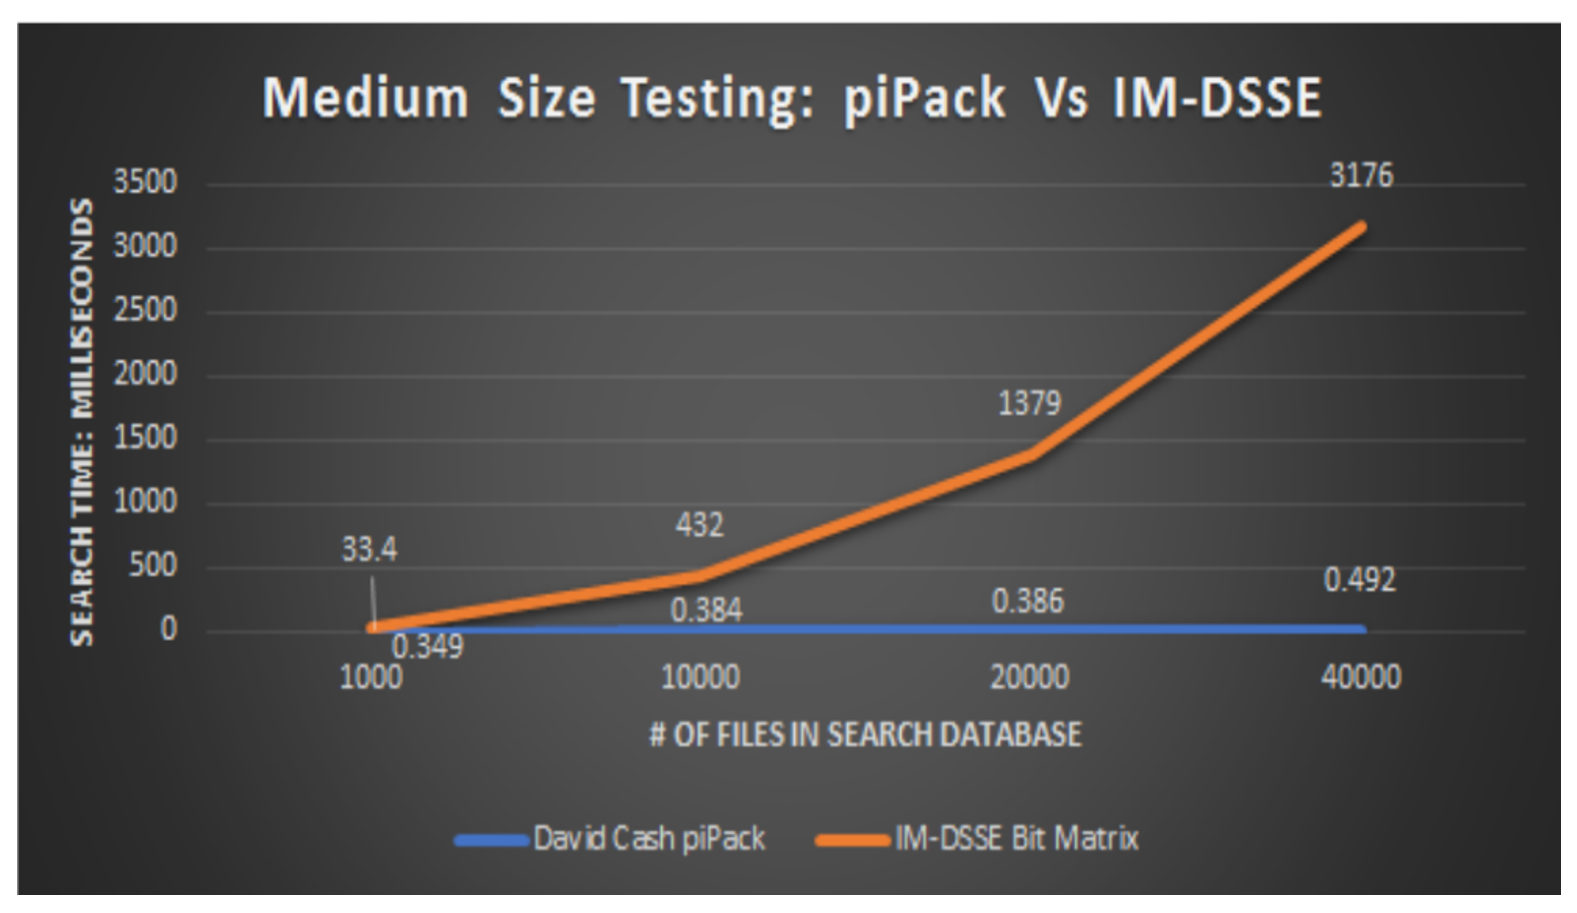
\includegraphics[width=0.8\textwidth]{Charts/medium_size.eps}
The medium size file benchmarking compares the results of IM-DSSE, David Cash Basic and David Cash piPack optimizations to compare the runtime speed of a search call to a database of 1000-40,000 files. Total number of keywords range up to 250,000. As we can see it is very clear that both version of David Cash scheme vastly outperform that of the IM-DSSE Bit Matrix. This makes sense, as we observe that the time complexity for IM-DSSE is $\mathcal{O} (n^2)$ where the search complexity of David Cash is closer to that of $\mathcal{O} (\log n)$. As file sizes increase the runspeed for IM-DSSE is substantially slower than David Cash. We will compare the basic to the optimization of piPack of David Cash in a later graph but we can clearly see here that David Cash has a vastly superior search speed, especially on larger data sets.

\subsection{IM-DSSE Bit Matrix Build time}
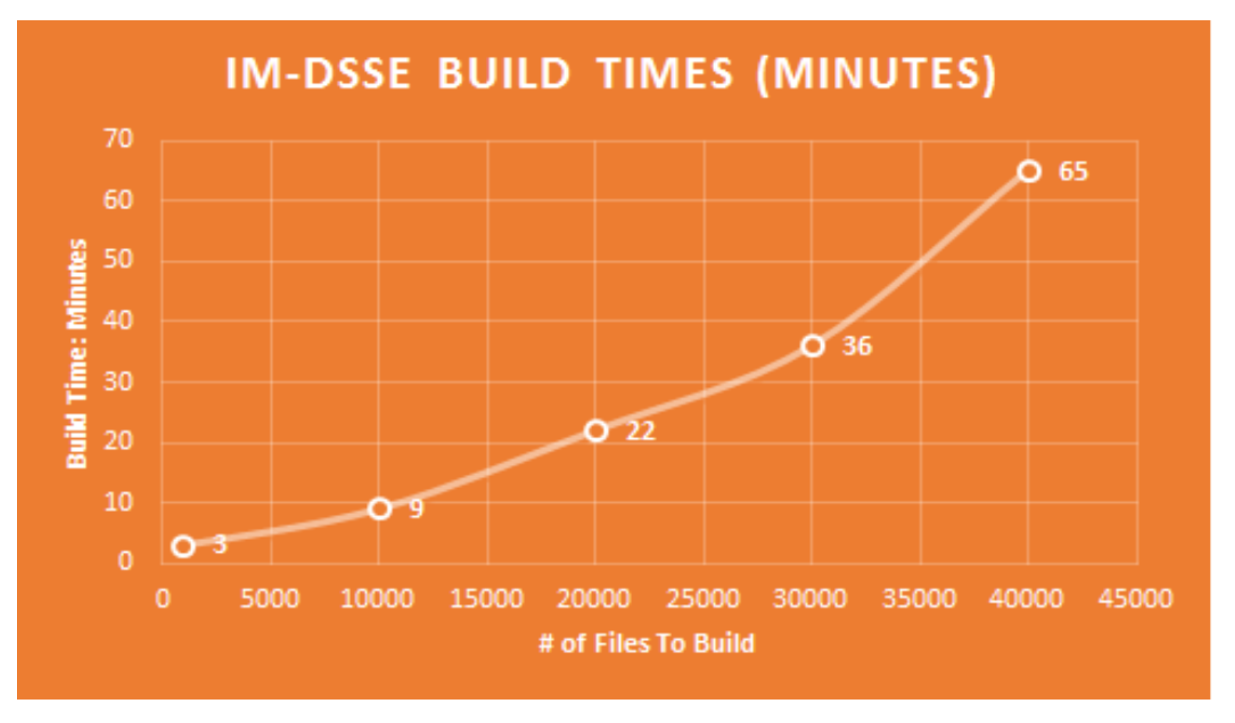
\includegraphics[width=1\textwidth]{Charts/time.eps}
The build time of the IM-DSSE Bit matrix scheme is also $\mathcal{O}(n^2)$ as it needs to create a key file pair with every single file and keyword found in the dataset. This takes a long time, and as a result our testing showed that the quadratic graph confirms that build speed. We did not graph it here but we also averaged out a build time, on the largest dataset of 40,000 files, to be around 2-3 minutes; thus vastly outperforming IM-DSSE at over an hour in build time.

\subsection{Small Data Single file benchmarking}
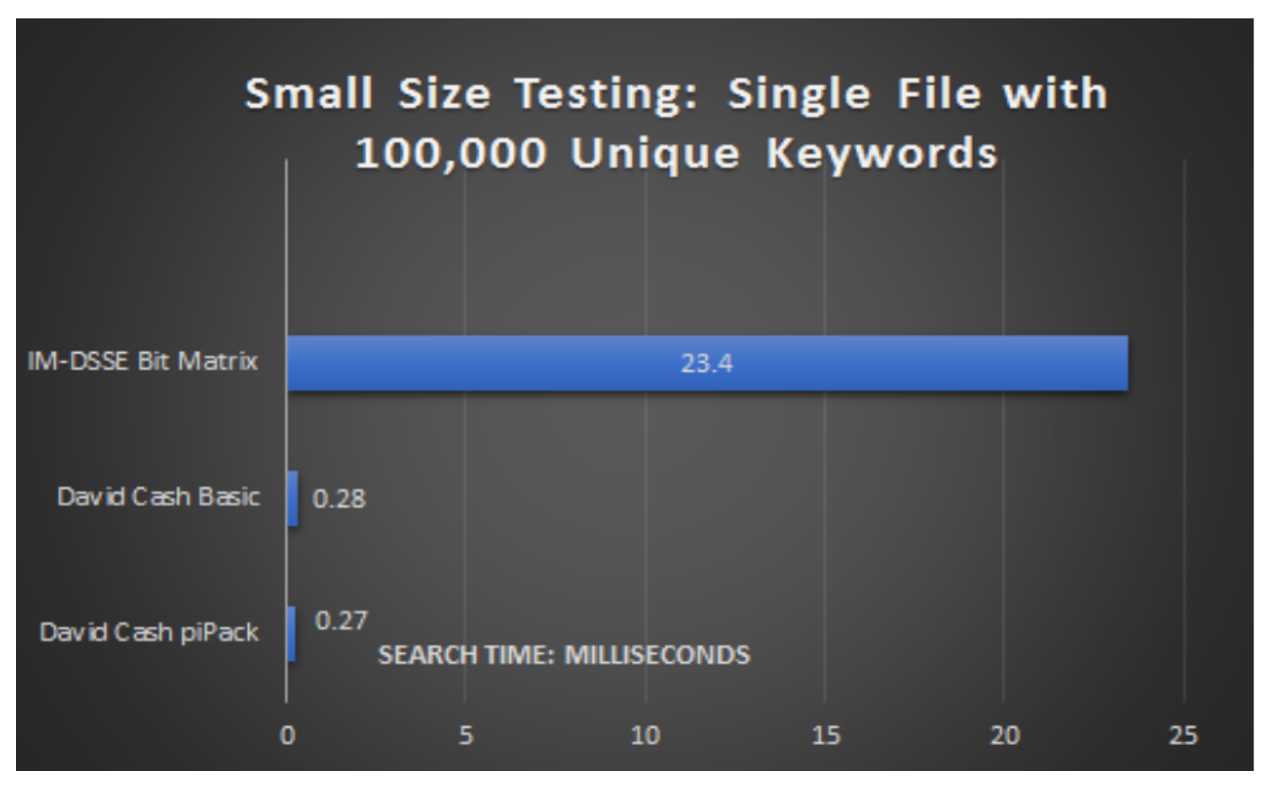
\includegraphics[width=.8\textwidth]{Charts/small.eps}
Similar to the large data set we also see that IM-DSSE is outperformed by David Cash substantially. The overhead of creating this key-file 2d matrix pair is simply much more expensive than the algorithm used by David Cash. The optimization between piPack and Basic is unsubstantial here as we are only working on a single file.
\subsection{DSSE Basic vs DSSE piPack Optimization Graph}
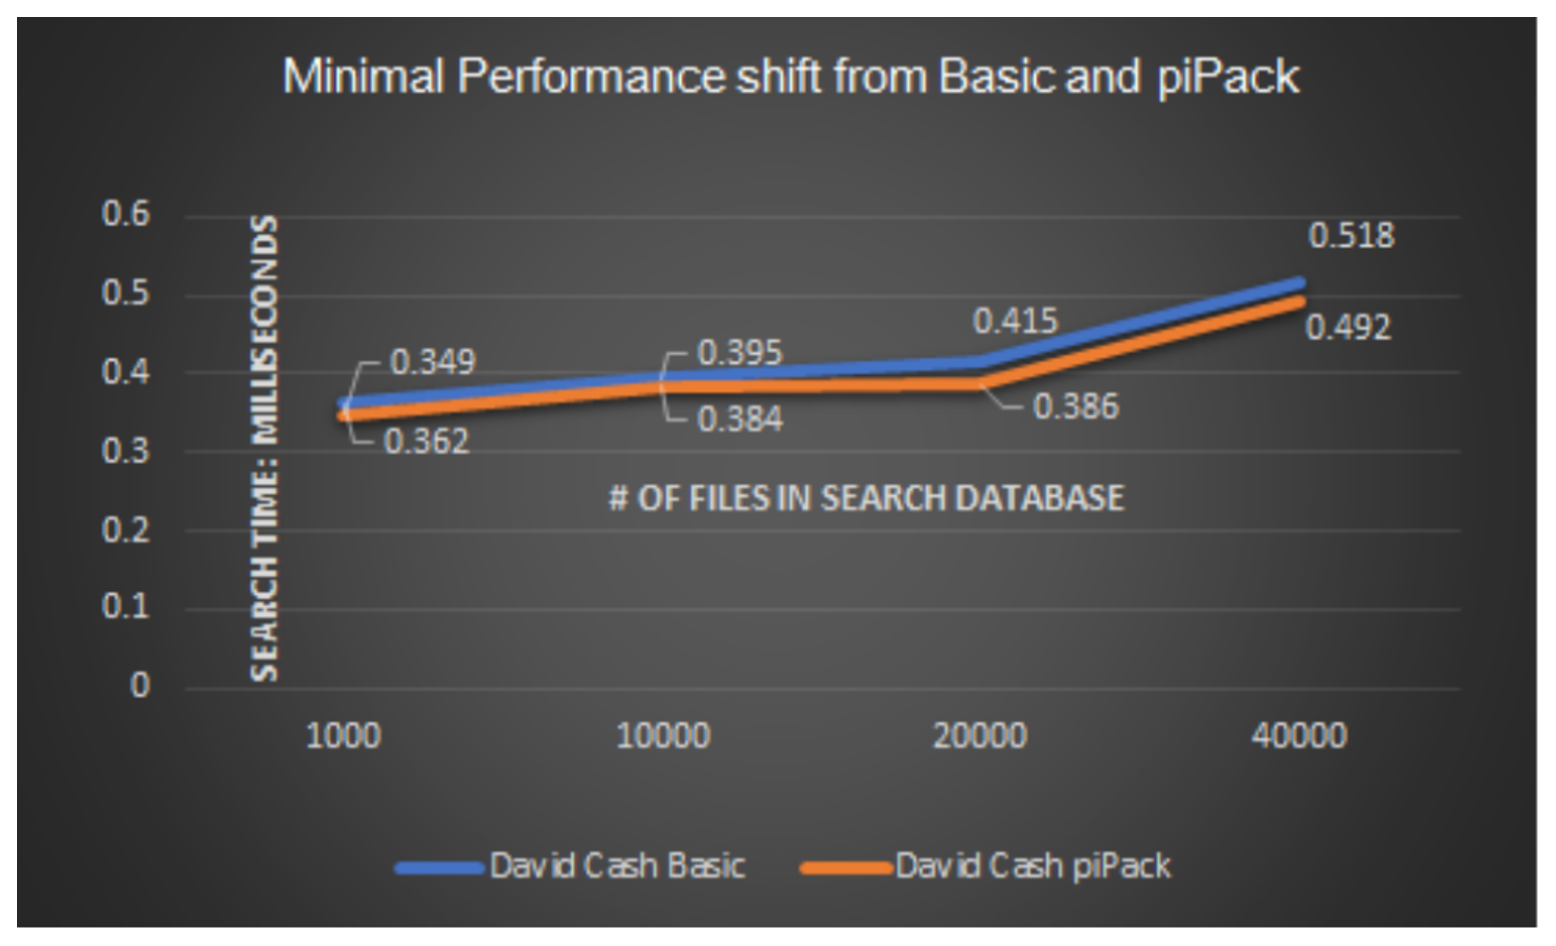
\includegraphics[width=1\textwidth]{Charts/Basic_Vs_piPack.eps}
From our results we believe that this graph is the most interesting to talk about. It is clear that there is a slight optimization between the piPack scheme over the basic. However it was not as large as we were expecting. We believe this is because the piPack scheme would better optimize disk access and data storage retrieval. However, for our testing purposes all the data is ran locally, therefore is on ram. Thus the piPack scheme does not provide the 
\subsection{Encrypted Size Comparison DSSE Basic VS IM-DSSE}
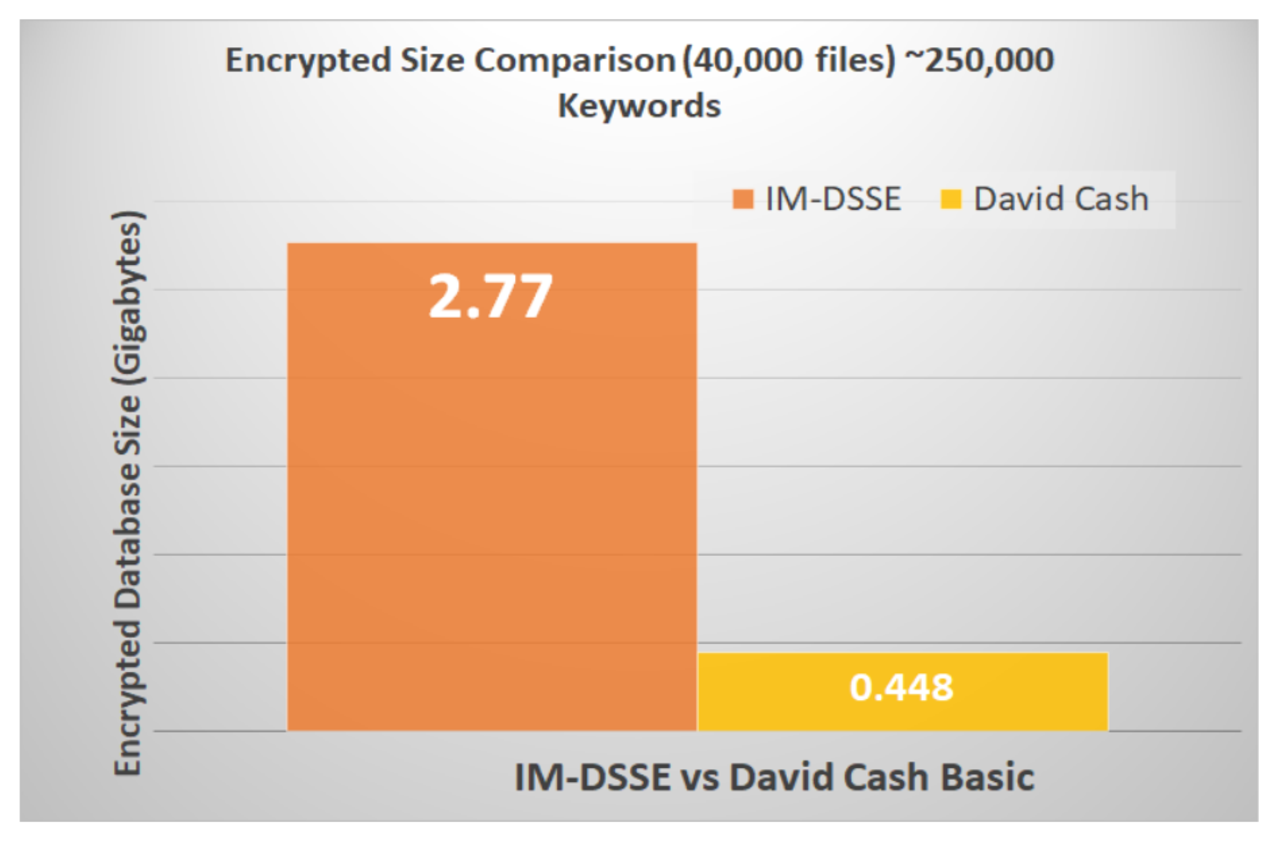
\includegraphics[width=.8\textwidth]{Charts/encrypt.eps}

The encrypted size comparison shows just how much larger the Encrypted Index is that is being searched through between cash and IM-DSSE. In addition to having a slower search time IM-DSSE indirectly composes its own larger dataset to search through because of its implementation of key-file pairs. Thus the size of the datasets are different. I expect this size to become even more drastic were we to test on a large database set such as the Wikipedia text data set.


	\subsection{Results}

% What did we learn?
% DSSE is very complex
% Benchmarking takes time
% In-memory data structures are fast but have limits

% Benchmark table
Our benchmark data showed that the scheme is very fast and can easily handle databases of over 40k files, which should suffice to store a normal user's emails or documents. We were unable to test larger databases because our test system ran out of memory --- one limitation of the current code is that it loads all data into memory before searching. We also transfer the entire database to the server in one message, which doesn't scale to large databases.

Interestingly, our benchmarks for $\Pi_\mathrm{pack}$ did not show much of a performance increase. There are a few possible explanations: maybe the block size we tested with was too small; maybe the optimization doesn't matter for an in-memory data structure; maybe the effect was swamped by the network overhead. We aren't sure. This deserves more attention.

We built a small demo web app for expo. This was a simple web frontend for the DSSE client which allowed people to search files in the database, and even to edit files. This was not strictly part of our project requirements, but it helped people see our project in action, and it aligned well with the spirit of our project, which was to show how privacy-preserving searchable encryption could be applied to the real world.

\subsubsection{Future work}

This section highlights some further areas of research. 
Searchable encryption is a relatively young field and so there is still a lot to discover.

\begin{itemize}
\item \textbf{Use a database.} In order to handle very large datasets that do not fit in main memory, the code would have to be modified to use an on-disk data structure. Some of the optimizations described in \cite{cash14}, particularly $\Pi_{\mathrm{ptr}}$ and $\Pi_{\mathrm{2lev}}$ seem like they are aimed at this use-case. Efficient on-disk data structures are a complex topic, but they are already well-studied. This is basically what databases are. We would be interested to see what would happen if you implemented $\Pi_{\mathrm{bas}}$ on top of an existing database library like \texttt{sqlite3} \cite{sqlite3}. We expect performance would be competitive without resorting to special tricks like $\Pi_{\mathrm{ptr}}$.

\item \textbf{Email integration.} One of our stretch goals was to build a daemon which periodically fetched emails and added them to the search index, to demonstrate a simple real-world use of DSSE. We didn't get to this, but it would still be an interesting experiment.

\item \textbf{Cloud platform integration.} Another stretch goal was to integrate with a cloud platform like Dropbox. This would require some rethinking of the DSSE scheme because we wouldn't be able to execute code on the server side, so the client would either have to fetch the whole encrypted index or the index would have to be broken up in some way.

\item \textbf{Storage-only server.} In the Cash-DSSE algorithm as described in the paper, the server performs the final decryption step, decrypting the file ids before handing them off to the client. This leaks a little information to the server over time. It would be better if the client performed all the decryption operations;  however, the Cash-DSSE scheme requires that the server to know the file ids it is returning in order to check the revocation set. To move decryption to the client would require an extra round-trip request. This needs further investigation.


\end{itemize}

\subsubsection{Conclusion}

We created an open-source implementation of the DSSE scheme described in \cite{cash14}
and were able to partially replicate the results.
Our benchmark data showed that the scheme is very fast and can easily handle databases of over 40k files, and we believe that with improvements to the code it should be able to handle even greater numbers.


% conclusions (per team member)
%\section{Conclusions and Reflections}
	% document include the answer to the conclusions and reflections questions

\chapter{Reflections}

% Each member will answer these questions ... no BS 
% Group Member 1
\subsection{Scott Russell}

\subsubsection{What technical information did you learn?}
There was allot of research done initially for this project. Security itself is a growing industry and to be able to maintain proficiencies we had to delve into some very modern crypto concepts. This is where the bulk of the focus went in the fall term, research. Winter term we were able to focus mostly on the implementation of the core DSSE scheme proposed by David Cash. His paper was the basis for our scheme, and our work as a whole. The concept of search-able encryption is extremely interesting to me as a security applied option and is considers some of the cutting edge technology in the security field. Being able to work with this new and research heavy work was very inspiring to future prospects as a graduate. Having this hands on experience has prepared me well for my future career as a Cyberwarfare officer.
\subsubsection{What non-technical information did you learn?}
A vast majority of this class was dealing with communication, coordination and work flow and supervision. It seemed much more toned toward a real world job situation. There was allot of scheduling that needed to be done that was difficult when trying to align free time between myself, Andrew Ekstedt, Scott Merrill, Andrew Emmott, Attila Yavuz and Thang Hoang. Trying to find a time that worked with all of us, or most of us, to meet and discuss progress and touch base, was difficult. This is akin to how scheduling can be in the work force where you have clients and teammates working remotely from across the world. These skills will be very useful in transitioning after graduation and I'm glad that this class brought up these important skills.

\subsubsection{What have you learned about project work?}
Scheduling is extremely difficult. With having cross town group mates, people getting sick, and in general life happening we weren't able to meet as a full team as often as I would of liked to. Working with a client was also an new experience for me. Instead of having a specified due date for each part of the project it was difficult for me to stay motivated. Therefore, I utilized mini-due dates that I would personally meet for work load. For example, "I will have this benchmark data done by Monday." Therefore I could use this small goals as plans in my OneNote to be able to continue progress week to week. As the term wrapped up I found it easier to stay focused as big final project deadlines began to loom closer. Now that we are finishing up the project I found that the entire experience of trying to manage a project is much less programming and much more communication than I initially thought.
\subsubsection{What have you learned about project management?}
Similar to project work managing the project has allot to do with setting and meeting short term goals to reach long term successes. You don't write a 50+ page Senior Capstone paper over night, well at least I hope no team did that! We spent the last 9 months working toward this goal. With small documents, each one adding to the final report, each page of code getting us closer to meeting requirements descriptions. Looking back at what we did I am proud of our team and how much we were able to accomplish in this time frame. If you had sat me down day one of capstone and told me I would be writing a 70 page paper by the end of the term with my team I would have given up. But because it was small increments, small successes and bit by bit we were able to come together to build something worth while.
\subsubsection{What have you learned about working in teams?}
Leadership and teamwork skills are paramount to success in a group environment. Being in the ROTC program here in campus we get drilled allot about the important to succeed or fail as a group. You may be an all star programmer, communicator and timely at work flow. But if you do it at the detriment to the rest of your team and leave them behind you will end up failing together. An analogy I like to refer to in this regard is "You have to step up to perform, but you are a single person on the team, be there supporting the rest at the plate." You have to step up to help your team complete their tasks, and they will do the same. It's a symbiotic relation.
\subsubsection{If you could do it all over, what would you do differently?}
I would have spent more time in the planning and preparing stage. This section of the work turned out to be extremely important in planning how we would be implementing different chunks of our project throughout the course of the assignment. We had some problems with falling behind our initial gantt chart that we prepared in fall term. We were able to adjust our project requirements to match the new scope and goal of capstone. Approval of this part with Attila turned out simple as he was very dynamic and adaptive to change as long as we maintained forward progress throughout the year.

% Group Member 2
\subsection{Group Member 2}

\subsubsection{What technical information did you learn?}
This project taught me a lot about cryptographic primitives, specifically dynamic searchable encryption. This was new to me and there was a large learning curve at the beginning of the project as much of the cryptography that was used I had not learned about before. This changed over the course of the years as I took more classes that address this.

\subsubsection{What non-technical information did you learn?}
Another major learning point from this project was how to work no a larger scale project than what OSU typically offers in other classes. The scope of this project, being over 3 terms, had us creating something much more complex than we normally can. Additionally, working as a group and learning how to break the project into different parts was new to me and I learned a lot from the experience.

\subsubsection{What have you learned about project work?}
Capstone did a great job teaching us about project work. One major emphasis that they placed upon us was to take good notes. We took notes for all meetings with out TA, Client, and during class. In addition to taking notes during meetings, we also took notes while working on our project. Making documentation for what we did, issues we ran across, and plans for the project going forward was a great learning experience.

\subsubsection{What have you learned about project management?}
This course had a heavy focus on project management. From the initial design to how to break down the project into digestible chunks was essential to our success. With a project on this scale it can be difficult to manage our time and goals appropriately to be successful and have a complete product by the time expo came around. This class does a great job of teaching us these points by having us experience these challenges first hand.

\subsubsection{What have you learned about working in teams?}
Working with others can always be a challenge. You need to be able to coordinate schedules, communicate effectively, work as a team, and learn about others strengths and weaknesses. By being a part of a project for the last 9 months, I was able to learn a lot about how to work well with a team. I thought this experience was one of the most valuable things that this course offers.

\subsubsection{If you could do it all over, what would you do differently?}
Looking back, now that the project is finished. The one thing I think I would have done differently would be to work with our client early to establish realistic expectations. We struggled in the beginning of the project because it had too many requirements than would be realistic for us to complete as a capstone project.

% Group Member 3
\subsection{Andrew Ekstedt}
\subsubsection{What technical information did you learn?}

Primarily, I learned about searchable encryption. I had never encountered the concept before this project, and now, having spent nine months working on it, I feel like I have a good knowledge of some of the ways it can be used, and some of its limitations. 

I also learned more about working in C++, which I didn't have much experience in prior to this capstone project. I'm still of the opinion that C++ is a poorly designed language - there is a lot of complexity and odd corner cases lurking to snare the uninitiated. I took some of the lessons learned about writing C++ and applied them to my class projects this term.

\subsubsection{What non-technical information did you learn?}


\subsubsection{What have you learned about project work?}
Don't depend on anyone.
% ...

\subsubsection{What have you learned about project management?}
I'm bad at project management.
% ...

\subsubsection{What have you learned about working in teams?}


\subsubsection{If you could do it all over, what would you do differently?}


% Expo poster!

%\begin{figure}
%\centering
%\includegraphics[angle=270,width=8in]{Charts/Capstone_Poster.eps}
%\caption{Capstone Poster chart}
%\label{figure:gantt}
%\end{figure}

% appendix 1: essential code listings

% References
\bibliography{main}{}


\end{document}
